\documentclass[12pt]{report}

%%
% to enumerate subsubsection
%%
\addtocounter{tocdepth}{3}
\setcounter{secnumdepth}{3}
% \usepackage{tgtermes}
\usepackage[a4paper, margin=1in]{geometry}
\usepackage[T1]{fontenc}
\usepackage[utf8]{inputenc}
\usepackage{graphicx} 
\usepackage{tikz}
\usepackage{amsmath, amssymb}
% \usepackage{indentfirst}
% \usepackage{cite}
\usepackage{natbib}
\usepackage[nameinlink,noabbrev]{cleveref}
\usepackage[capposition=top]{floatrow}
\usepackage{float}
\usepackage{caption}
\usepackage{xfrac}
\usepackage{braket}
\usepackage[toc,page]{appendix}
\usepackage{tabularx}
% \usepackage{hyperref}
% \usepackage{physics}

%%
% to enumerate subsubsection
%%
\addtocounter{tocdepth}{3}
\setcounter{secnumdepth}{3}

% Snippet
\newcommand{\BSM}{Black--Scholes--Merton }
\newcommand{\lnorm}{log-normally }
\newcommand{\bmotion}{Brownian Motion }
\newcommand{\stvar}{stochastic variable }
\newcommand{\wienpro}{Wiener process }
\newcommand{\markpro}{Markov process }

% 
% Bunch of new commands
% 
% brownian motion
\newcommand{\dBm}{dW\left(t\right)}
\newcommand{\dpoiss}{dq\left(t\right)}
\newcommand{\DBm}{\delta{W\left(t\right)}}
\newcommand{\Bm}{W\left(t\right)}
\newcommand{\Bmsub}[1]{W_{#1}\left(t\right)}
\newcommand{\Dt}{\Delta t} 
\newcommand{\Bmdist}{\DBm \sim N \left( 0, \Dt \right)}
\newcommand{\ft}{f\left(t, \Bm \right)}
\newcommand{\E}{\mathop{\mathbb{E}}}
\newcommand{\ct}{c\left(t, x\right)}
\newcommand{\dcx}{\frac{\delta\ct}{\delta x}}
\newcommand{\dciix}{\frac{\delta^2\ct}{\delta x^2}}
\newcommand{\dct}{\frac{\delta\ct}{\delta t}}
\newcommand{\N}[1]{N\left(#1\right)}
\newcommand{\dsub}[1]{d_{#1}\left(\Dt, x\right)}
\newcommand{\call}[2]{c\left( #1, #2\right)}
% % about stock
\newcommand{\St}{S\left(t\right)}
\newcommand{\Vt}{V\left(t\right)}
\newcommand{\Si}{S\left(0\right)}
\newcommand{\dSt}{dS\left(t\right)}
\newcommand{\DSt}{\Delta S\left(t\right)}
\newcommand{\dSr}{\frac{\dSt}{\St}}
\newcommand{\DSr}{\frac{\DSt}{\St}}
\newcommand{\Scontinuous}{\St = \Si e^{\sigma\Bm + \left(\alpha - \frac{1}{2 \sigma^2}\right)t}}
\newcommand{\Itobmdiff}{d\ft = \left[\frac{\partial \ft }{\partial t} + \frac{1}{2} \frac{\partial ^2\ft }{\partial x^2}\right]dt + \frac{\partial \ft}{\partial x} \dBm}
\newcommand{\Scontinousdiff}{d\St &= \alpha \St dt + \sigma \St \dBm}
\newcommand{\Scontinuousrate}{\dSr &= \alpha dt + \sigma \dBm}
 \newcommand{\Sdiscretediff}{d\St &= \alpha \St \Dt + \sigma \St \dBm}
\newcommand{\Sshort}{\Si e^{X}}
\newcommand{\CCRdist}{X \sim N\left(\left(\alpha - \frac{1}{2}\sigma^2\right)t, \sigma^2 t\right)}
\newcommand{\Sdiscreterate}{\DSr &= \alpha \Delta t + \sigma \DBm}
\newcommand{\Sdiscreterateexp}{\E \DSr = \alpha \Dt}
\newcommand{\Sdiscreteratevar}{var \DSr = \sigma ^2 \Dt}
\newcommand{\Sdiscreteratedist}{\DSr \sim N\left(\alpha\Dt, \sigma\Dt\right)}
\newcommand{\Sexp}{\E\St = \Si e^{\alpha t}}
\newcommand{\Svar}{var\St = \Si^2 e^{2\alpha t}\left(e^{\sigma^2 t} - 1\right)}
\newcommand{\Sshortt}{\St = \Si e^{X t}}
\newcommand{\CCRt}{X = \frac{1}{t} \ln{\frac{\St}{\Si}}}
\newcommand{\CCRtdist}{X \sim N\left(\alpha - \frac{\sigma^2}{2}, \frac{\sigma^2}{t}\right)}
\newcommand{\BSMpde}{\dct + r x \dcx + \frac{1}{2} \sigma^2 x^2 \dciix = r\ct}
\newcommand{\BSMeq}[1]{r\call{t}{#1} = \frac{\partial \call{t}{#1}}{\partial t} + r #1 \frac{\partial \call{t}{#1}}{\partial #1} + \frac{1}{2} \sigma ^2 #1 ^2 \frac{\partial ^2 \call{t}{#1}}{\partial #1 ^2}}
\newcommand{\BSMGreeks}[1]{r\call{t}{#1} = \Theta + r #1 \Delta + \frac{1}{2} \sigma ^2 #1 ^2 \Gamma}
\newcommand{\BSMsol}{\ct &= x\N{\dsub{+}} - K e^{-r\Dt} \N{\dsub{-}}}
\newcommand{\dpm}{\dsub{\pm} &= \frac{1}{\sigma\sqrt{\Dt}} \left[\log\frac{x}{K} + \left(r \pm \frac{\sigma^2}{2}\Dt\right)\right]}

% CIR Stock price Stochastic process
\newcommand{\HSVstock}{
  d\St &= \alpha \St dt + \sqrt{\Vt} \St d \Bmsub{S}
}

% CIR Stock price Stochastic process
\newcommand{\HSVstockriskless}{
  d\St &= r \St dt + \sqrt{\Vt} \St d \Bmsub{S}
}

% CIR volatility
\newcommand{\HSVvol}{
  d\Vt &= \kappa\left(\theta - \Vt \right) dt + \sigma \sqrt{\Vt} d \Bmsub{V}
}


% CIR volatility
\newcommand{\HSVvolriskless}{
  d\Vt &= \kappa^{*} \left(\theta^{*} - \Vt \right) dt + \sigma \sqrt{\Vt} d \Bmsub{V}
}

\newcommand{\dportfolio}{dX\left(t\right) &= \Delta\left(t\right) d\St + r \left(X\left(t\right) - \Delta\left(t\right) \St \right) dt}

\usepackage{Sweave}
\begin{document}
\Sconcordance{concordance:index.tex:index.Rnw:%
1 6 1}
\Sconcordance{concordance:index.tex:./preamble/usepackage.Rnw:ofs 7:%
1 21 1}
\Sconcordance{concordance:index.tex:./preamble/misc.Rnw:ofs 29:%
1 6 1}
\Sconcordance{concordance:index.tex:./preamble/snippet.Rnw:ofs 36:%
1 7 1}
\Sconcordance{concordance:index.tex:./preamble/formula.Rnw:ofs 44:%
1 71 1}
\Sconcordance{concordance:index.tex:index.Rnw:ofs 116:%
12 1 1 1 0 24 1}
\Sconcordance{concordance:index.tex:./methodology.Rnw:ofs 143:%
1 485 1}
\Sconcordance{concordance:index.tex:index.Rnw:ofs 629:%
39 12 1}

\tableofcontents{}



%%%%%%%%%%%%%%%%%%%%%%%%%%%%%%%%%%%%%%%%%%%%%%%%%%%%%%%%%%%%%%%%%%%%%%%%%%%%%%%%
%
%  CHAPTER: Introduction
%
%%%%%%%%%%%%%%%%%%%%%%%%%%%%%%%%%%%%%%%%%%%%%%%%%%%%%%%%%%%%%%%%%%%%%%%%%%%%%%%%
\chapter*{Introduction}
\label{cha:Introduction}
\addcontentsline{toc}{chapter}{Introduction}

Talk about what is done to price a vanilla option throuhout the BSM method.
How does the BSM model is fair under its assumption. What about if we are going beyond ?
How perfomant is it ? 
What about other model such as \ldots ?

Using R. \cite{R}
% \SweaveInput{upstream}
% \SweaveInput{underlying}
% \SweaveInput{BSM}
% \SweaveInput{models}
%%%%%%%%%%%%%%%%%%%%%%%%%%%%%%%%%%%%%%%%%%%%%%%%%%%%%%%%%%%%%%%%%%%%%%%%%%%%%%%%
%
%  CHAPTER:Methodology
%
%%%%%%%%%%%%%%%%%%%%%%%%%%%%%%%%%%%%%%%%%%%%%%%%%%%%%%%%%%%%%%%%%%%%%%%%%%%%%%%%
\chapter{Methodology}
\label{cha:Methodology}


\section{Overview}
\label{sec:methodology:overview}

The objective of this master thesis is to measure the performances of the Black-Scholes-Merton pricing method when the assumption of normality for the log-returns distribution is not met.

In order to measure such performances, I will (i) compute the options price by using in turn the models BSM, Merton mixed jump-diffusion and Heston stochastic volatility models. 
Thereafter, I will (ii) compare the implied volatility of those computed prices split by maturities and by models.
Finally, I will (iii) construct delta-neutral portfolios to measure the hedging performance of the aforementioned models.

Instead of exclusively using market data, whether to gather option prices or to build the delta-neutral portfolio, I will rather construct some theoretical based algorithm.
Depending on the framework to explore, the option prices will be computed either by using the BSM equation, if the underlying process relates to a geometric Brownian motion or by using the method developed by \citet{heston1993}, it the underlying process relates to the model MJD or HSV.
To assess the delta-neutral portfolio, I will need time series to measure its evolution across time. those series will be simulated based on the theories developed by \citet{merton76} and \citet{heston1993} in order to respectively obtain paths with jumps and others with stochastic volatility.
Consequently, I have built some functions in the R language to perform those tasks. \cref{t:methodology:r} is a summary of a few of them used in that chapter and in the analysis. More details on them are given in appendix \cref{R functions catalogue}.

\begin{table}[ht]
  \begin{tabularx}{\textwidth}{llX}
    \hline
    Function name & Arguments & Purpose \\
    \hline
    bsm\_call & $\left \{ S(0), T, k, r, \sigma \right \}$ & Compute the BSM price of an option \\
    mjd\_call & $\left \{ S(0), T, k, r, \lambda, \mu, \delta \sigma \right \}$ & Compute the Merton price of an option \\
    hsv\_call & $\left \{ S(0), T, k, r, V(0), \theta, \kappa, \sigma, \rho \right \}$ & Compute the heston price of an option \\
    bsm\_ts & $\left \{ S(0), T, \sigma, \alpha, dt \right \}$ & Simulate BSM time series \\
    mjd\_ts & $\left \{ S(0), T, \sigma, \alpha, \lambda, \mu, \delta dt \right \}$ & Simulate MJD time series \\
    hsv\_ts & $\left \{ S(0), T, V(0), \alpha, \rho, \kappa, \theta, \sigma, dt \right \}$ & Simulate HSV time series \\
  \end{tabularx}
  \caption{R functions dealing with options and time series}
  \label{t:methodology:r}
\end{table}

Even though I won't construct my hedge directly on market data, I need those data to calibrate the parameters to pass into the functions listed in \cref{t:methodology:r}.
Therefore, the functions with the objective to provide european call price will be calibrated with the Apple european call market data while, to stay consistent, the functions that simulate time series will be benchmarked using the Apple stock data available on the market.
This process of calibration is fully explained at \cref{sec:methodology:calibration}.


%%%%%%%%%%%%%%%%%%%%%%%%%%%%%%%%%%%%%%%%%%%%%%%%%%%%%%%%%%%%%%%%%%%%%%%%%%%%%%%%
% SECTION: calibration
%%%%%%%%%%%%%%%%%%%%%%%%%%%%%%%%%%%%%%%%%%%%%%%%%%%%%%%%%%%%%%%%%%%%%%%%%%%%%%%%
\section{Calibration}
\label{sec:methodology:calibration}

Whenever one deals with functions aimed to reproduce some real-life experiments, the calibration process is crucial because it gives to the functions the capacity to act within appropriate boundaries.

The process of calibration which will be applied in the current section concerns two distinctive groups of parameters. 
Those intended to the functions that compute the European call price and those used by the functions that simulate the hypothetical stock market movements.
Consequently, the methods to calibrate both kinds of arguments differ, mainly because the options prices calculation must be performed under risk-neutral environment and the delta hedging is measured on time-series evolving under a risk-averse world.

To do so, I am going to use the available option price data to calibrate the arguments aimed to the functions that compute the price of the latter. 
Whilst I am going to use the stock's historical data to estimate the right values for the time-series output-related functions.
The option market prices and stock data were downloaded using the package \textit{quantmod}, developed by \citet{quantmod} which uses Yahoo! finance as provider. The datasets so downloaded are available in appendix \ref{cha:appendix:market}.

\Cref{sub:methodology:calibration:option} explains how I am going to operate for the options' parameters, whereas \cref{sub:methodology:calibration:asset} shows the procedure I am going to follow for the assets simulations' arguments.


%%%%%%%%%%%%%%%%%%%%%%%%%%%%%%%%%%%%%%%%%%%%%%%%%%%%%%%%%%%%%%%%%%%%%%%%%%%%%%%%
% SUBSECTION: Option prices' calibration
%%%%%%%%%%%%%%%%%%%%%%%%%%%%%%%%%%%%%%%%%%%%%%%%%%%%%%%%%%%%%%%%%%%%%%%%%%%%%%%%
\subsection{Option prices based calibration}
\label{sub:methodology:calibration:option}

In accordance to \citet{heston1993} and \citet{criso2015}, provided that the characteristic functions of the MJD and HSV models are known, the European call option price of such underlying processes can be computed using \cref{eq:other:call:heston}.
Although known, these characteristics functions (\cref{eq:other:merton:psi,eq:other:heston:psi}) need some parameters to work and these parameters need appropriates values to best fit with what is observed in reality.
That is why both functions need to be benchmarked with referential values before being used.

To do so, I am going to apply the same method followed by \citet{criso2015}, namely, iteratively minimizing the difference between the options market prices and those generated by the functions that compute the option prices based on the characteristic functions.
As the market data comes with a large number of maturities and stikes, \cref{t:methodology:maturity,t:methodology:strike} list those considered during the analysis.

\begin{table}[ht]
\centering
\begin{tabular}{lllllll}
  63 & 91 & 126 & 154 & 182 & 245 & 399 \\
\end{tabular}
\caption{Taking into account maturities during calibration stage} 
\label{t:methodology:maturity}
\end{table}

\begin{table}[ht]
\centering
\begin{tabular}{llllllllll}
  130 & 140 & 150 & 160 & 170 & 180 & 190 & 200 & 210 & 220 \\  
\end{tabular}
\caption{Taking into account strikes during calibration stage} 
\label{t:methodology:strike}
\end{table}

The optimization method used is the least-square non-linear analysis. 
To work, such a method need (i) a function that returns dummy data, (ii) a dataset of data to serve as a template, (iii) a cost function to minimize and (iv) the parameters to optimize.

The functions that return the artificial data are those exhibited in \cref{t:methodology:r}, that is to say, \textit{mjd\_call} and \textit{hsv\_call} for the computation of call price using MJD and HSV, respectively.
The dataset template is the one in \cref{t:market:option} (see appendix \ref{cha:appendix:market}).
While the cost function is given by \cref{eq:methodology:cost}, the parameters to assess depend on the underlying model (either MJD or HSV).

\begin{align}
 &\left(C_{K,T}^{mkt} - C_{K,T}^{h|m}(arguments)\right)^2
 \label{eq:methodology:cost}\\
 \forall &K \in \{130, 140, 150, 160, 170, 180, 190, 200, 210, 220\}, \notag\\
 &T \in \left \{63, 91, 126, 154, 182, 245, 399\right \}\notag 
\end{align}
Where the subscripts $K$ and $T$ respectively stand for strike price and maturity date, while the superscripts $mkt$ denotes the "market price" and $h|m$ refers to either Heston or Merton process based prices.

Consequently, the \cref{eq:methodology:cost} is that to be minimized using the least-square non-linear analysis, for all strikes and maturities.
The output of this process will eventually be the calibrated arguments that maximize the performance of the model with respect to what is observed in the reality.

One difficulty when dealing with such an algorithm is that the least-square non-linear approach may return several best-fit sets of arguments due to the existence of multiple local minima in the cost function.
Therefore, in order to choose among all the outputs provided by the optimization method, I will select those that ensure that the pricing function gives the most of its returns within the bid-ask spread of the option data, as shown by \cref{eq:methodology:bidask}.

\begin{align}
  C_{bid}^{mkt} \leq C_{K,T}^{h|m}(arguments)  \leq C_{ask}^{mkt}
 \label{eq:methodology:bidask}
\end{align}

Even though the cost function to be optimized is the same for both HSV and MJD pricing option procedures, the arguments to calibrate are different. \cref{sub:methodology:calibration:merton,sub:methodology:calibration:heston} respectively illustrate the  MJD and HSV calibration process and results.

%%%%%%%%%%%%%%%%%%%%%%%%%%%%%%%%%%%%%%%%%%%%%%%%%%%%%%%%%%%%%%%%%%%%%%%%%%%%%%%%
% SUBSECTION: Asset prices based calibration
%%%%%%%%%%%%%%%%%%%%%%%%%%%%%%%%%%%%%%%%%%%%%%%%%%%%%%%%%%%%%%%%%%%%%%%%%%%%%%%%

\subsection{Asset prices based calibration}
\label{sub:methodology:calibration:asset}

In order to calibrate the parameters to pass to the MJD and HSV model, to generate all the dummy times series that will serve for the analysis of the delta hedging, I am going to use the historical market data on the Apple stock as a template.

To perform such an upstream analysis, I will use an approximation method to estimate the arguments with which the distribution of the log-returns generated by both MJD and HSV models better fit the density curve of the historical log-return.
The list of arguments to estimate will be smaller than the one needed to option calibration because I will start with the set of the already assessed parameters from options data and only (re)calibrate those risk-neutralized.

To get the historical data, I will once more use the package \textit{quantmod}, developed by \citet{quantmod} which uses Yahoo! finance as a provider. The dataset so downloaded is available in appendix \ref{cha:appendix:apple} and concerns the daily stock price from 18th May 2017 to 18th May 2018.
\cref{p:methodology:density:aapl} shows the density curve generated by the log-return of the historical data.

\begin{figure}[ht]
  \centering
  % Created by tikzDevice version 0.11 on 2018-07-31 15:58:40
% !TEX encoding = UTF-8 Unicode

  \caption{Historical Apple stock Log-returns distribution}
  \floatfoot{The above densities function is constructed over the historical data of the Apple share of stock price evolution from 18th May 2017 to 18th May 2018.
  
  }
  \label{p:methodology:density:aapl}
\end{figure}


The procedures to calibrate the arguments for MJD and HSV processes are respectively explained at \cref{sub:methodology:calibration:merton,sub:methodology:calibration:heston}.


% SUBSECTION: Merton's model calibration

\subsection{Merton's model calibration}
\label{sub:methodology:calibration:merton}


% SUBSECTION: Heston's model calibration

\subsection{Heston's model calibration}
\label{sub:methodology:calibration:heston}

\subsubsection*{Calibration of parameters for option pricing}

In order to use the function \textit{hsv\_call} based on \cref{eq:other:call:heston} to compute the price of European call options on an underlying with increments driven by the HSV model, the parameters $(V(0), \kappa, \theta, \sigma, \rho)$ must be calibrated with respect to the available option market data.
Consequently, the so estimated parameters will be in line with the risk-neutral measure, or more specifically $\kappa$ and $\theta$, which are the only ones adapted to make \cref{eq:other:hsvvol:riskless} risk-neutral.

To do so, I am going to use the aforementioned least-square non-linear analysis together with data on Apple call option as a template.
In that respect, the theoretical models to calibrate are given by \crefrange{eq:other:call:heston}{eq:other:call:heston:pi2} along with \cref{eq:other:heston:psi}, implemented by the R function \textit{hsv\_call}.

Moreover, to stay in a range of acceptable values, the parameters of the HSV model should lie between some defined boundaries. 

De facto, the mean-reversion speed ($\kappa$), the long-run variance ($\theta$) and the volatility of the volatility ($\sigma$) need to take values that together respect the Feller's condition (see \cref{sub:other:heston:feller}). 
Additionally, $\sigma$ should range between 0 and 1 and, according to \citet{cristo2015} $\kappa$ should be positive to avoid mean aversion.
Although the correlation coefficient $\rho$ may take any value from $[-1, 1]$, typically the correlation between the stock price increments and their intrinsic volatility is negative. Consequently, I set the borders of $\rho$ as being $]0, -1[$.

According to those constraints and due to the presence of multiple local minima, the \textit{lsqnonlin} function returns the \cref{t:methodology:call:heston:estimate1} as the whole sets of parameters that make the function \textit{hsv\_call} better fit with reality.

\begin{table}[ht]
\centering
\begin{tabular}{rrrrr}
  \hline
v0 & theta & sigma & rho & kappa \\ 
  \hline
0.03835 & 0.05144 & 0.30882 & -0.40228 & 1.99821 \\ 
  0.03851 & 0.05142 & 0.29539 & -0.49338 & 1.99931 \\ 
  0.03850 & 0.05241 & 0.30601 & -0.59979 & 1.99843 \\ 
  0.03774 & 0.04832 & 0.30687 & -0.40213 & 3.00036 \\ 
  0.03827 & 0.04954 & 0.40690 & -0.40189 & 3.00011 \\ 
  0.03883 & 0.04798 & 0.30747 & -0.50211 & 3.00015 \\ 
  0.03910 & 0.04948 & 0.40736 & -0.50193 & 3.00005 \\ 
  0.03695 & 0.04703 & 0.30697 & -0.40288 & 4.00092 \\ 
  0.04449 & 0.04443 & 0.40682 & -0.40289 & 4.00079 \\ 
  0.03798 & 0.04872 & 0.50379 & -0.39878 & 4.00106 \\ 
  0.04091 & 0.04651 & 0.40705 & -0.50227 & 4.00097 \\ 
  0.03740 & 0.04754 & 0.30583 & -0.60126 & 4.00096 \\ 
  0.03890 & 0.04792 & 0.40565 & -0.60086 & 4.00091 \\ 
  0.03661 & 0.04604 & 0.30659 & -0.40295 & 5.00152 \\ 
  0.04034 & 0.04547 & 0.40591 & -0.40298 & 5.00153 \\ 
  0.04111 & 0.04558 & 0.50652 & -0.40298 & 5.00144 \\ 
  0.04034 & 0.04720 & 0.60647 & -0.40250 & 5.00138 \\ 
  0.03921 & 0.04709 & 0.50753 & -0.50170 & 5.00152 \\ 
  0.03789 & 0.04656 & 0.30488 & -0.80072 & 5.00164 \\ 
   \hline
\end{tabular}
\caption{Best estimates for HSV call option model} 
\label{t:methodology:call:heston:estimate1}
\end{table}

Otherwise, The set \ref{eq:methodology:arg:heston:riskneutral} is the one making respond the model the best with what is observed in reality.
Indeed when passing that set to the R function \textit{call\_heston}, for all strikes of \cref{t:methodology:strike} and maturities of \cref{t:methodology:maturity}, more than $70\%$ of the so generated prices are within the bid-ask spread of the Apple option historical data.

\begin{align}
  \left \{
  \begin{array}{lcl}
    V(0) &= &0.03798218, \\
    \theta &= &0.04871543, \\
    \sigma &= &0.50378803, \\
    \rho &= &-0.39877827, \\
    \kappa &= &4.00105546 
  \end{array}
  \right \}  
  \label{eq:methodology:arg:heston:riskneutral}
\end{align}

\cref{{p:methodology:impliedvol:aapl:heston}} confronts the blue colored volatility smiles computed from market data, with those dotted in red, calculated from the function \textit{hsv\_call}, which takes the items of the set \ref{eq:methodology:arg:heston:riskneutral} as parameters.

\begin{figure}[H]
  \centering
  % Created by tikzDevice version 0.11 on 2018-07-20 21:55:59
% !TEX encoding = UTF-8 Unicode
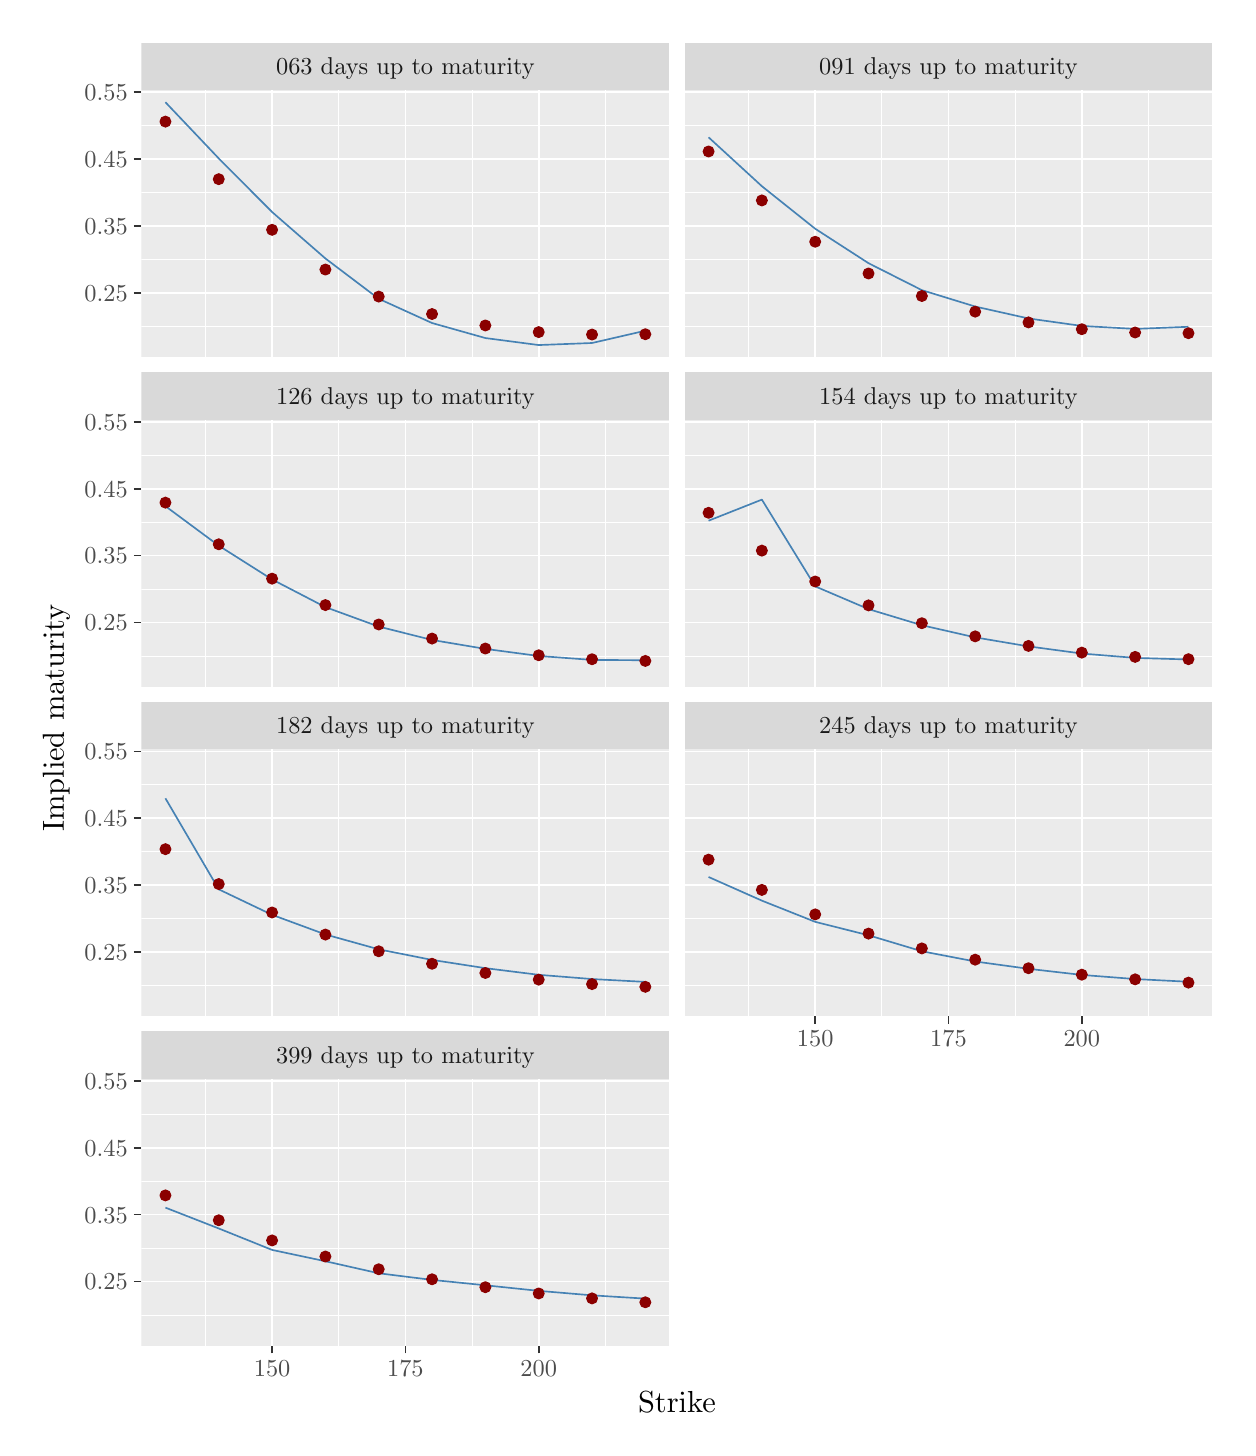
\begin{tikzpicture}[x=1pt,y=1pt]
\definecolor{fillColor}{RGB}{255,255,255}
\path[use as bounding box,fill=fillColor,fill opacity=0.00] (0,0) rectangle (433.62,505.89);
\begin{scope}
\path[clip] (  0.00,  0.00) rectangle (433.62,505.89);
\definecolor{drawColor}{RGB}{255,255,255}
\definecolor{fillColor}{RGB}{255,255,255}

\path[draw=drawColor,line width= 0.6pt,line join=round,line cap=round,fill=fillColor] (  0.00,  0.00) rectangle (433.62,505.89);
\end{scope}
\begin{scope}
\path[clip] ( 41.11,386.81) rectangle (231.87,483.33);
\definecolor{fillColor}{gray}{0.92}

\path[fill=fillColor] ( 41.11,386.81) rectangle (231.87,483.33);
\definecolor{drawColor}{RGB}{255,255,255}

\path[draw=drawColor,line width= 0.3pt,line join=round] ( 41.11,397.93) --
	(231.87,397.93);

\path[draw=drawColor,line width= 0.3pt,line join=round] ( 41.11,422.11) --
	(231.87,422.11);

\path[draw=drawColor,line width= 0.3pt,line join=round] ( 41.11,446.28) --
	(231.87,446.28);

\path[draw=drawColor,line width= 0.3pt,line join=round] ( 41.11,470.45) --
	(231.87,470.45);

\path[draw=drawColor,line width= 0.3pt,line join=round] ( 64.23,386.81) --
	( 64.23,483.33);

\path[draw=drawColor,line width= 0.3pt,line join=round] (112.40,386.81) --
	(112.40,483.33);

\path[draw=drawColor,line width= 0.3pt,line join=round] (160.57,386.81) --
	(160.57,483.33);

\path[draw=drawColor,line width= 0.3pt,line join=round] (208.74,386.81) --
	(208.74,483.33);

\path[draw=drawColor,line width= 0.6pt,line join=round] ( 41.11,410.02) --
	(231.87,410.02);

\path[draw=drawColor,line width= 0.6pt,line join=round] ( 41.11,434.19) --
	(231.87,434.19);

\path[draw=drawColor,line width= 0.6pt,line join=round] ( 41.11,458.37) --
	(231.87,458.37);

\path[draw=drawColor,line width= 0.6pt,line join=round] ( 41.11,482.54) --
	(231.87,482.54);

\path[draw=drawColor,line width= 0.6pt,line join=round] ( 88.32,386.81) --
	( 88.32,483.33);

\path[draw=drawColor,line width= 0.6pt,line join=round] (136.49,386.81) --
	(136.49,483.33);

\path[draw=drawColor,line width= 0.6pt,line join=round] (184.66,386.81) --
	(184.66,483.33);
\definecolor{drawColor}{RGB}{70,130,180}

\path[draw=drawColor,line width= 0.6pt,line join=round] ( 49.78,478.94) --
	( 69.05,458.63) --
	( 88.32,439.27) --
	(107.59,422.48) --
	(126.85,407.92) --
	(146.12,399.16) --
	(165.39,393.73) --
	(184.66,391.20) --
	(203.93,391.94) --
	(223.19,396.38);
\definecolor{drawColor}{RGB}{139,0,0}
\definecolor{fillColor}{RGB}{139,0,0}

\path[draw=drawColor,line width= 0.4pt,line join=round,line cap=round,fill=fillColor] ( 49.78,471.94) circle (  1.96);

\path[draw=drawColor,line width= 0.4pt,line join=round,line cap=round,fill=fillColor] ( 69.05,451.14) circle (  1.96);

\path[draw=drawColor,line width= 0.4pt,line join=round,line cap=round,fill=fillColor] ( 88.32,432.84) circle (  1.96);

\path[draw=drawColor,line width= 0.4pt,line join=round,line cap=round,fill=fillColor] (107.59,418.48) circle (  1.96);

\path[draw=drawColor,line width= 0.4pt,line join=round,line cap=round,fill=fillColor] (126.85,408.72) circle (  1.96);

\path[draw=drawColor,line width= 0.4pt,line join=round,line cap=round,fill=fillColor] (146.12,402.41) circle (  1.96);

\path[draw=drawColor,line width= 0.4pt,line join=round,line cap=round,fill=fillColor] (165.39,398.28) circle (  1.96);

\path[draw=drawColor,line width= 0.4pt,line join=round,line cap=round,fill=fillColor] (184.66,395.88) circle (  1.96);

\path[draw=drawColor,line width= 0.4pt,line join=round,line cap=round,fill=fillColor] (203.93,394.99) circle (  1.96);

\path[draw=drawColor,line width= 0.4pt,line join=round,line cap=round,fill=fillColor] (223.19,395.11) circle (  1.96);
\end{scope}
\begin{scope}
\path[clip] ( 41.11,267.74) rectangle (231.87,364.25);
\definecolor{fillColor}{gray}{0.92}

\path[fill=fillColor] ( 41.11,267.74) rectangle (231.87,364.25);
\definecolor{drawColor}{RGB}{255,255,255}

\path[draw=drawColor,line width= 0.3pt,line join=round] ( 41.11,278.86) --
	(231.87,278.86);

\path[draw=drawColor,line width= 0.3pt,line join=round] ( 41.11,303.03) --
	(231.87,303.03);

\path[draw=drawColor,line width= 0.3pt,line join=round] ( 41.11,327.20) --
	(231.87,327.20);

\path[draw=drawColor,line width= 0.3pt,line join=round] ( 41.11,351.38) --
	(231.87,351.38);

\path[draw=drawColor,line width= 0.3pt,line join=round] ( 64.23,267.74) --
	( 64.23,364.25);

\path[draw=drawColor,line width= 0.3pt,line join=round] (112.40,267.74) --
	(112.40,364.25);

\path[draw=drawColor,line width= 0.3pt,line join=round] (160.57,267.74) --
	(160.57,364.25);

\path[draw=drawColor,line width= 0.3pt,line join=round] (208.74,267.74) --
	(208.74,364.25);

\path[draw=drawColor,line width= 0.6pt,line join=round] ( 41.11,290.95) --
	(231.87,290.95);

\path[draw=drawColor,line width= 0.6pt,line join=round] ( 41.11,315.12) --
	(231.87,315.12);

\path[draw=drawColor,line width= 0.6pt,line join=round] ( 41.11,339.29) --
	(231.87,339.29);

\path[draw=drawColor,line width= 0.6pt,line join=round] ( 41.11,363.46) --
	(231.87,363.46);

\path[draw=drawColor,line width= 0.6pt,line join=round] ( 88.32,267.74) --
	( 88.32,364.25);

\path[draw=drawColor,line width= 0.6pt,line join=round] (136.49,267.74) --
	(136.49,364.25);

\path[draw=drawColor,line width= 0.6pt,line join=round] (184.66,267.74) --
	(184.66,364.25);
\definecolor{drawColor}{RGB}{70,130,180}

\path[draw=drawColor,line width= 0.6pt,line join=round] ( 49.78,332.98) --
	( 69.05,318.71) --
	( 88.32,306.50) --
	(107.59,296.51) --
	(126.85,289.47) --
	(146.12,284.64) --
	(165.39,281.41) --
	(184.66,278.85) --
	(203.93,277.43) --
	(223.19,277.30);
\definecolor{drawColor}{RGB}{139,0,0}
\definecolor{fillColor}{RGB}{139,0,0}

\path[draw=drawColor,line width= 0.4pt,line join=round,line cap=round,fill=fillColor] ( 49.78,334.26) circle (  1.96);

\path[draw=drawColor,line width= 0.4pt,line join=round,line cap=round,fill=fillColor] ( 69.05,319.20) circle (  1.96);

\path[draw=drawColor,line width= 0.4pt,line join=round,line cap=round,fill=fillColor] ( 88.32,306.79) circle (  1.96);

\path[draw=drawColor,line width= 0.4pt,line join=round,line cap=round,fill=fillColor] (107.59,297.24) circle (  1.96);

\path[draw=drawColor,line width= 0.4pt,line join=round,line cap=round,fill=fillColor] (126.85,290.23) circle (  1.96);

\path[draw=drawColor,line width= 0.4pt,line join=round,line cap=round,fill=fillColor] (146.12,285.14) circle (  1.96);

\path[draw=drawColor,line width= 0.4pt,line join=round,line cap=round,fill=fillColor] (165.39,281.54) circle (  1.96);

\path[draw=drawColor,line width= 0.4pt,line join=round,line cap=round,fill=fillColor] (184.66,279.10) circle (  1.96);

\path[draw=drawColor,line width= 0.4pt,line join=round,line cap=round,fill=fillColor] (203.93,277.67) circle (  1.96);

\path[draw=drawColor,line width= 0.4pt,line join=round,line cap=round,fill=fillColor] (223.19,277.06) circle (  1.96);
\end{scope}
\begin{scope}
\path[clip] ( 41.11,148.66) rectangle (231.87,245.18);
\definecolor{fillColor}{gray}{0.92}

\path[fill=fillColor] ( 41.11,148.66) rectangle (231.87,245.18);
\definecolor{drawColor}{RGB}{255,255,255}

\path[draw=drawColor,line width= 0.3pt,line join=round] ( 41.11,159.78) --
	(231.87,159.78);

\path[draw=drawColor,line width= 0.3pt,line join=round] ( 41.11,183.96) --
	(231.87,183.96);

\path[draw=drawColor,line width= 0.3pt,line join=round] ( 41.11,208.13) --
	(231.87,208.13);

\path[draw=drawColor,line width= 0.3pt,line join=round] ( 41.11,232.30) --
	(231.87,232.30);

\path[draw=drawColor,line width= 0.3pt,line join=round] ( 64.23,148.66) --
	( 64.23,245.18);

\path[draw=drawColor,line width= 0.3pt,line join=round] (112.40,148.66) --
	(112.40,245.18);

\path[draw=drawColor,line width= 0.3pt,line join=round] (160.57,148.66) --
	(160.57,245.18);

\path[draw=drawColor,line width= 0.3pt,line join=round] (208.74,148.66) --
	(208.74,245.18);

\path[draw=drawColor,line width= 0.6pt,line join=round] ( 41.11,171.87) --
	(231.87,171.87);

\path[draw=drawColor,line width= 0.6pt,line join=round] ( 41.11,196.04) --
	(231.87,196.04);

\path[draw=drawColor,line width= 0.6pt,line join=round] ( 41.11,220.21) --
	(231.87,220.21);

\path[draw=drawColor,line width= 0.6pt,line join=round] ( 41.11,244.39) --
	(231.87,244.39);

\path[draw=drawColor,line width= 0.6pt,line join=round] ( 88.32,148.66) --
	( 88.32,245.18);

\path[draw=drawColor,line width= 0.6pt,line join=round] (136.49,148.66) --
	(136.49,245.18);

\path[draw=drawColor,line width= 0.6pt,line join=round] (184.66,148.66) --
	(184.66,245.18);
\definecolor{drawColor}{RGB}{70,130,180}

\path[draw=drawColor,line width= 0.6pt,line join=round] ( 49.78,227.41) --
	( 69.05,194.52) --
	( 88.32,185.32) --
	(107.59,178.22) --
	(126.85,172.85) --
	(146.12,169.02) --
	(165.39,166.04) --
	(184.66,163.64) --
	(203.93,162.11) --
	(223.19,161.08);
\definecolor{drawColor}{RGB}{139,0,0}
\definecolor{fillColor}{RGB}{139,0,0}

\path[draw=drawColor,line width= 0.4pt,line join=round,line cap=round,fill=fillColor] ( 49.78,209.04) circle (  1.96);

\path[draw=drawColor,line width= 0.4pt,line join=round,line cap=round,fill=fillColor] ( 69.05,196.43) circle (  1.96);

\path[draw=drawColor,line width= 0.4pt,line join=round,line cap=round,fill=fillColor] ( 88.32,186.16) circle (  1.96);

\path[draw=drawColor,line width= 0.4pt,line join=round,line cap=round,fill=fillColor] (107.59,178.18) circle (  1.96);

\path[draw=drawColor,line width= 0.4pt,line join=round,line cap=round,fill=fillColor] (126.85,172.14) circle (  1.96);

\path[draw=drawColor,line width= 0.4pt,line join=round,line cap=round,fill=fillColor] (146.12,167.63) circle (  1.96);

\path[draw=drawColor,line width= 0.4pt,line join=round,line cap=round,fill=fillColor] (165.39,164.30) circle (  1.96);

\path[draw=drawColor,line width= 0.4pt,line join=round,line cap=round,fill=fillColor] (184.66,161.90) circle (  1.96);

\path[draw=drawColor,line width= 0.4pt,line join=round,line cap=round,fill=fillColor] (203.93,160.28) circle (  1.96);

\path[draw=drawColor,line width= 0.4pt,line join=round,line cap=round,fill=fillColor] (223.19,159.30) circle (  1.96);
\end{scope}
\begin{scope}
\path[clip] ( 41.11, 29.59) rectangle (231.87,126.10);
\definecolor{fillColor}{gray}{0.92}

\path[fill=fillColor] ( 41.11, 29.59) rectangle (231.87,126.10);
\definecolor{drawColor}{RGB}{255,255,255}

\path[draw=drawColor,line width= 0.3pt,line join=round] ( 41.11, 40.71) --
	(231.87, 40.71);

\path[draw=drawColor,line width= 0.3pt,line join=round] ( 41.11, 64.88) --
	(231.87, 64.88);

\path[draw=drawColor,line width= 0.3pt,line join=round] ( 41.11, 89.05) --
	(231.87, 89.05);

\path[draw=drawColor,line width= 0.3pt,line join=round] ( 41.11,113.22) --
	(231.87,113.22);

\path[draw=drawColor,line width= 0.3pt,line join=round] ( 64.23, 29.59) --
	( 64.23,126.10);

\path[draw=drawColor,line width= 0.3pt,line join=round] (112.40, 29.59) --
	(112.40,126.10);

\path[draw=drawColor,line width= 0.3pt,line join=round] (160.57, 29.59) --
	(160.57,126.10);

\path[draw=drawColor,line width= 0.3pt,line join=round] (208.74, 29.59) --
	(208.74,126.10);

\path[draw=drawColor,line width= 0.6pt,line join=round] ( 41.11, 52.79) --
	(231.87, 52.79);

\path[draw=drawColor,line width= 0.6pt,line join=round] ( 41.11, 76.97) --
	(231.87, 76.97);

\path[draw=drawColor,line width= 0.6pt,line join=round] ( 41.11,101.14) --
	(231.87,101.14);

\path[draw=drawColor,line width= 0.6pt,line join=round] ( 41.11,125.31) --
	(231.87,125.31);

\path[draw=drawColor,line width= 0.6pt,line join=round] ( 88.32, 29.59) --
	( 88.32,126.10);

\path[draw=drawColor,line width= 0.6pt,line join=round] (136.49, 29.59) --
	(136.49,126.10);

\path[draw=drawColor,line width= 0.6pt,line join=round] (184.66, 29.59) --
	(184.66,126.10);
\definecolor{drawColor}{RGB}{70,130,180}

\path[draw=drawColor,line width= 0.6pt,line join=round] ( 49.78, 79.51) --
	( 69.05, 71.98) --
	( 88.32, 64.23) --
	(107.59, 60.14) --
	(126.85, 55.79) --
	(146.12, 53.40) --
	(165.39, 51.45) --
	(184.66, 49.44) --
	(203.93, 47.82) --
	(223.19, 46.63);
\definecolor{drawColor}{RGB}{139,0,0}
\definecolor{fillColor}{RGB}{139,0,0}

\path[draw=drawColor,line width= 0.4pt,line join=round,line cap=round,fill=fillColor] ( 49.78, 83.93) circle (  1.96);

\path[draw=drawColor,line width= 0.4pt,line join=round,line cap=round,fill=fillColor] ( 69.05, 74.95) circle (  1.96);

\path[draw=drawColor,line width= 0.4pt,line join=round,line cap=round,fill=fillColor] ( 88.32, 67.66) circle (  1.96);

\path[draw=drawColor,line width= 0.4pt,line join=round,line cap=round,fill=fillColor] (107.59, 61.84) circle (  1.96);

\path[draw=drawColor,line width= 0.4pt,line join=round,line cap=round,fill=fillColor] (126.85, 57.24) circle (  1.96);

\path[draw=drawColor,line width= 0.4pt,line join=round,line cap=round,fill=fillColor] (146.12, 53.62) circle (  1.96);

\path[draw=drawColor,line width= 0.4pt,line join=round,line cap=round,fill=fillColor] (165.39, 50.76) circle (  1.96);

\path[draw=drawColor,line width= 0.4pt,line join=round,line cap=round,fill=fillColor] (184.66, 48.50) circle (  1.96);

\path[draw=drawColor,line width= 0.4pt,line join=round,line cap=round,fill=fillColor] (203.93, 46.72) circle (  1.96);

\path[draw=drawColor,line width= 0.4pt,line join=round,line cap=round,fill=fillColor] (223.19, 45.31) circle (  1.96);
\end{scope}
\begin{scope}
\path[clip] (237.37,386.81) rectangle (428.12,483.33);
\definecolor{fillColor}{gray}{0.92}

\path[fill=fillColor] (237.37,386.81) rectangle (428.12,483.33);
\definecolor{drawColor}{RGB}{255,255,255}

\path[draw=drawColor,line width= 0.3pt,line join=round] (237.37,397.93) --
	(428.12,397.93);

\path[draw=drawColor,line width= 0.3pt,line join=round] (237.37,422.11) --
	(428.12,422.11);

\path[draw=drawColor,line width= 0.3pt,line join=round] (237.37,446.28) --
	(428.12,446.28);

\path[draw=drawColor,line width= 0.3pt,line join=round] (237.37,470.45) --
	(428.12,470.45);

\path[draw=drawColor,line width= 0.3pt,line join=round] (260.49,386.81) --
	(260.49,483.33);

\path[draw=drawColor,line width= 0.3pt,line join=round] (308.66,386.81) --
	(308.66,483.33);

\path[draw=drawColor,line width= 0.3pt,line join=round] (356.83,386.81) --
	(356.83,483.33);

\path[draw=drawColor,line width= 0.3pt,line join=round] (405.00,386.81) --
	(405.00,483.33);

\path[draw=drawColor,line width= 0.6pt,line join=round] (237.37,410.02) --
	(428.12,410.02);

\path[draw=drawColor,line width= 0.6pt,line join=round] (237.37,434.19) --
	(428.12,434.19);

\path[draw=drawColor,line width= 0.6pt,line join=round] (237.37,458.37) --
	(428.12,458.37);

\path[draw=drawColor,line width= 0.6pt,line join=round] (237.37,482.54) --
	(428.12,482.54);

\path[draw=drawColor,line width= 0.6pt,line join=round] (284.57,386.81) --
	(284.57,483.33);

\path[draw=drawColor,line width= 0.6pt,line join=round] (332.74,386.81) --
	(332.74,483.33);

\path[draw=drawColor,line width= 0.6pt,line join=round] (380.91,386.81) --
	(380.91,483.33);
\definecolor{drawColor}{RGB}{70,130,180}

\path[draw=drawColor,line width= 0.6pt,line join=round] (246.04,466.27) --
	(265.30,448.60) --
	(284.57,433.23) --
	(303.84,420.78) --
	(323.11,411.04) --
	(342.38,405.12) --
	(361.64,400.81) --
	(380.91,398.11) --
	(400.18,397.03) --
	(419.45,397.80);
\definecolor{drawColor}{RGB}{139,0,0}
\definecolor{fillColor}{RGB}{139,0,0}

\path[draw=drawColor,line width= 0.4pt,line join=round,line cap=round,fill=fillColor] (246.04,461.14) circle (  1.96);

\path[draw=drawColor,line width= 0.4pt,line join=round,line cap=round,fill=fillColor] (265.30,443.46) circle (  1.96);

\path[draw=drawColor,line width= 0.4pt,line join=round,line cap=round,fill=fillColor] (284.57,428.53) circle (  1.96);

\path[draw=drawColor,line width= 0.4pt,line join=round,line cap=round,fill=fillColor] (303.84,417.06) circle (  1.96);

\path[draw=drawColor,line width= 0.4pt,line join=round,line cap=round,fill=fillColor] (323.11,408.92) circle (  1.96);

\path[draw=drawColor,line width= 0.4pt,line join=round,line cap=round,fill=fillColor] (342.38,403.27) circle (  1.96);

\path[draw=drawColor,line width= 0.4pt,line join=round,line cap=round,fill=fillColor] (361.64,399.38) circle (  1.96);

\path[draw=drawColor,line width= 0.4pt,line join=round,line cap=round,fill=fillColor] (380.91,396.93) circle (  1.96);

\path[draw=drawColor,line width= 0.4pt,line join=round,line cap=round,fill=fillColor] (400.18,395.74) circle (  1.96);

\path[draw=drawColor,line width= 0.4pt,line join=round,line cap=round,fill=fillColor] (419.45,395.48) circle (  1.96);
\end{scope}
\begin{scope}
\path[clip] (237.37,267.74) rectangle (428.12,364.25);
\definecolor{fillColor}{gray}{0.92}

\path[fill=fillColor] (237.37,267.74) rectangle (428.12,364.25);
\definecolor{drawColor}{RGB}{255,255,255}

\path[draw=drawColor,line width= 0.3pt,line join=round] (237.37,278.86) --
	(428.12,278.86);

\path[draw=drawColor,line width= 0.3pt,line join=round] (237.37,303.03) --
	(428.12,303.03);

\path[draw=drawColor,line width= 0.3pt,line join=round] (237.37,327.20) --
	(428.12,327.20);

\path[draw=drawColor,line width= 0.3pt,line join=round] (237.37,351.38) --
	(428.12,351.38);

\path[draw=drawColor,line width= 0.3pt,line join=round] (260.49,267.74) --
	(260.49,364.25);

\path[draw=drawColor,line width= 0.3pt,line join=round] (308.66,267.74) --
	(308.66,364.25);

\path[draw=drawColor,line width= 0.3pt,line join=round] (356.83,267.74) --
	(356.83,364.25);

\path[draw=drawColor,line width= 0.3pt,line join=round] (405.00,267.74) --
	(405.00,364.25);

\path[draw=drawColor,line width= 0.6pt,line join=round] (237.37,290.95) --
	(428.12,290.95);

\path[draw=drawColor,line width= 0.6pt,line join=round] (237.37,315.12) --
	(428.12,315.12);

\path[draw=drawColor,line width= 0.6pt,line join=round] (237.37,339.29) --
	(428.12,339.29);

\path[draw=drawColor,line width= 0.6pt,line join=round] (237.37,363.46) --
	(428.12,363.46);

\path[draw=drawColor,line width= 0.6pt,line join=round] (284.57,267.74) --
	(284.57,364.25);

\path[draw=drawColor,line width= 0.6pt,line join=round] (332.74,267.74) --
	(332.74,364.25);

\path[draw=drawColor,line width= 0.6pt,line join=round] (380.91,267.74) --
	(380.91,364.25);
\definecolor{drawColor}{RGB}{70,130,180}

\path[draw=drawColor,line width= 0.6pt,line join=round] (246.04,327.73) --
	(265.30,335.35) --
	(284.57,304.00) --
	(303.84,295.78) --
	(323.11,289.96) --
	(342.38,285.57) --
	(361.64,282.32) --
	(380.91,279.73) --
	(400.18,278.15) --
	(419.45,277.58);
\definecolor{drawColor}{RGB}{139,0,0}
\definecolor{fillColor}{RGB}{139,0,0}

\path[draw=drawColor,line width= 0.4pt,line join=round,line cap=round,fill=fillColor] (246.04,330.58) circle (  1.96);

\path[draw=drawColor,line width= 0.4pt,line join=round,line cap=round,fill=fillColor] (265.30,316.92) circle (  1.96);

\path[draw=drawColor,line width= 0.4pt,line join=round,line cap=round,fill=fillColor] (284.57,305.76) circle (  1.96);

\path[draw=drawColor,line width= 0.4pt,line join=round,line cap=round,fill=fillColor] (303.84,297.13) circle (  1.96);

\path[draw=drawColor,line width= 0.4pt,line join=round,line cap=round,fill=fillColor] (323.11,290.69) circle (  1.96);

\path[draw=drawColor,line width= 0.4pt,line join=round,line cap=round,fill=fillColor] (342.38,285.94) circle (  1.96);

\path[draw=drawColor,line width= 0.4pt,line join=round,line cap=round,fill=fillColor] (361.64,282.48) circle (  1.96);

\path[draw=drawColor,line width= 0.4pt,line join=round,line cap=round,fill=fillColor] (380.91,280.06) circle (  1.96);

\path[draw=drawColor,line width= 0.4pt,line join=round,line cap=round,fill=fillColor] (400.18,278.52) circle (  1.96);

\path[draw=drawColor,line width= 0.4pt,line join=round,line cap=round,fill=fillColor] (419.45,277.69) circle (  1.96);
\end{scope}
\begin{scope}
\path[clip] (237.37,148.66) rectangle (428.12,245.18);
\definecolor{fillColor}{gray}{0.92}

\path[fill=fillColor] (237.37,148.66) rectangle (428.12,245.18);
\definecolor{drawColor}{RGB}{255,255,255}

\path[draw=drawColor,line width= 0.3pt,line join=round] (237.37,159.78) --
	(428.12,159.78);

\path[draw=drawColor,line width= 0.3pt,line join=round] (237.37,183.96) --
	(428.12,183.96);

\path[draw=drawColor,line width= 0.3pt,line join=round] (237.37,208.13) --
	(428.12,208.13);

\path[draw=drawColor,line width= 0.3pt,line join=round] (237.37,232.30) --
	(428.12,232.30);

\path[draw=drawColor,line width= 0.3pt,line join=round] (260.49,148.66) --
	(260.49,245.18);

\path[draw=drawColor,line width= 0.3pt,line join=round] (308.66,148.66) --
	(308.66,245.18);

\path[draw=drawColor,line width= 0.3pt,line join=round] (356.83,148.66) --
	(356.83,245.18);

\path[draw=drawColor,line width= 0.3pt,line join=round] (405.00,148.66) --
	(405.00,245.18);

\path[draw=drawColor,line width= 0.6pt,line join=round] (237.37,171.87) --
	(428.12,171.87);

\path[draw=drawColor,line width= 0.6pt,line join=round] (237.37,196.04) --
	(428.12,196.04);

\path[draw=drawColor,line width= 0.6pt,line join=round] (237.37,220.21) --
	(428.12,220.21);

\path[draw=drawColor,line width= 0.6pt,line join=round] (237.37,244.39) --
	(428.12,244.39);

\path[draw=drawColor,line width= 0.6pt,line join=round] (284.57,148.66) --
	(284.57,245.18);

\path[draw=drawColor,line width= 0.6pt,line join=round] (332.74,148.66) --
	(332.74,245.18);

\path[draw=drawColor,line width= 0.6pt,line join=round] (380.91,148.66) --
	(380.91,245.18);
\definecolor{drawColor}{RGB}{70,130,180}

\path[draw=drawColor,line width= 0.6pt,line join=round] (246.04,198.99) --
	(265.30,190.44) --
	(284.57,182.78) --
	(303.84,177.93) --
	(323.11,172.15) --
	(342.38,168.45) --
	(361.64,165.81) --
	(380.91,163.60) --
	(400.18,162.11) --
	(419.45,161.13);
\definecolor{drawColor}{RGB}{139,0,0}
\definecolor{fillColor}{RGB}{139,0,0}

\path[draw=drawColor,line width= 0.4pt,line join=round,line cap=round,fill=fillColor] (246.04,205.25) circle (  1.96);

\path[draw=drawColor,line width= 0.4pt,line join=round,line cap=round,fill=fillColor] (265.30,194.32) circle (  1.96);

\path[draw=drawColor,line width= 0.4pt,line join=round,line cap=round,fill=fillColor] (284.57,185.47) circle (  1.96);

\path[draw=drawColor,line width= 0.4pt,line join=round,line cap=round,fill=fillColor] (303.84,178.53) circle (  1.96);

\path[draw=drawColor,line width= 0.4pt,line join=round,line cap=round,fill=fillColor] (323.11,173.18) circle (  1.96);

\path[draw=drawColor,line width= 0.4pt,line join=round,line cap=round,fill=fillColor] (342.38,169.11) circle (  1.96);

\path[draw=drawColor,line width= 0.4pt,line join=round,line cap=round,fill=fillColor] (361.64,166.02) circle (  1.96);

\path[draw=drawColor,line width= 0.4pt,line join=round,line cap=round,fill=fillColor] (380.91,163.69) circle (  1.96);

\path[draw=drawColor,line width= 0.4pt,line join=round,line cap=round,fill=fillColor] (400.18,162.00) circle (  1.96);

\path[draw=drawColor,line width= 0.4pt,line join=round,line cap=round,fill=fillColor] (419.45,160.81) circle (  1.96);
\end{scope}
\begin{scope}
\path[clip] ( 41.11,126.10) rectangle (231.87,143.16);
\definecolor{fillColor}{gray}{0.85}

\path[fill=fillColor] ( 41.11,126.10) rectangle (231.87,143.16);
\definecolor{drawColor}{gray}{0.10}

\node[text=drawColor,anchor=base,inner sep=0pt, outer sep=0pt, scale=  0.88] at (136.49,131.60) {399 days up to maturity};
\end{scope}
\begin{scope}
\path[clip] ( 41.11,245.18) rectangle (231.87,262.24);
\definecolor{fillColor}{gray}{0.85}

\path[fill=fillColor] ( 41.11,245.18) rectangle (231.87,262.24);
\definecolor{drawColor}{gray}{0.10}

\node[text=drawColor,anchor=base,inner sep=0pt, outer sep=0pt, scale=  0.88] at (136.49,250.68) {182 days up to maturity};
\end{scope}
\begin{scope}
\path[clip] (237.37,245.18) rectangle (428.12,262.24);
\definecolor{fillColor}{gray}{0.85}

\path[fill=fillColor] (237.37,245.18) rectangle (428.12,262.24);
\definecolor{drawColor}{gray}{0.10}

\node[text=drawColor,anchor=base,inner sep=0pt, outer sep=0pt, scale=  0.88] at (332.74,250.68) {245 days up to maturity};
\end{scope}
\begin{scope}
\path[clip] ( 41.11,364.25) rectangle (231.87,381.31);
\definecolor{fillColor}{gray}{0.85}

\path[fill=fillColor] ( 41.11,364.25) rectangle (231.87,381.31);
\definecolor{drawColor}{gray}{0.10}

\node[text=drawColor,anchor=base,inner sep=0pt, outer sep=0pt, scale=  0.88] at (136.49,369.75) {126 days up to maturity};
\end{scope}
\begin{scope}
\path[clip] (237.37,364.25) rectangle (428.12,381.31);
\definecolor{fillColor}{gray}{0.85}

\path[fill=fillColor] (237.37,364.25) rectangle (428.12,381.31);
\definecolor{drawColor}{gray}{0.10}

\node[text=drawColor,anchor=base,inner sep=0pt, outer sep=0pt, scale=  0.88] at (332.74,369.75) {154 days up to maturity};
\end{scope}
\begin{scope}
\path[clip] ( 41.11,483.33) rectangle (231.87,500.39);
\definecolor{fillColor}{gray}{0.85}

\path[fill=fillColor] ( 41.11,483.33) rectangle (231.87,500.39);
\definecolor{drawColor}{gray}{0.10}

\node[text=drawColor,anchor=base,inner sep=0pt, outer sep=0pt, scale=  0.88] at (136.49,488.83) {063 days up to maturity};
\end{scope}
\begin{scope}
\path[clip] (237.37,483.33) rectangle (428.12,500.39);
\definecolor{fillColor}{gray}{0.85}

\path[fill=fillColor] (237.37,483.33) rectangle (428.12,500.39);
\definecolor{drawColor}{gray}{0.10}

\node[text=drawColor,anchor=base,inner sep=0pt, outer sep=0pt, scale=  0.88] at (332.74,488.83) {091 days up to maturity};
\end{scope}
\begin{scope}
\path[clip] (  0.00,  0.00) rectangle (433.62,505.89);
\definecolor{drawColor}{gray}{0.20}

\path[draw=drawColor,line width= 0.6pt,line join=round] ( 88.32, 26.84) --
	( 88.32, 29.59);

\path[draw=drawColor,line width= 0.6pt,line join=round] (136.49, 26.84) --
	(136.49, 29.59);

\path[draw=drawColor,line width= 0.6pt,line join=round] (184.66, 26.84) --
	(184.66, 29.59);
\end{scope}
\begin{scope}
\path[clip] (  0.00,  0.00) rectangle (433.62,505.89);
\definecolor{drawColor}{gray}{0.30}

\node[text=drawColor,anchor=base,inner sep=0pt, outer sep=0pt, scale=  0.88] at ( 88.32, 18.58) {150};

\node[text=drawColor,anchor=base,inner sep=0pt, outer sep=0pt, scale=  0.88] at (136.49, 18.58) {175};

\node[text=drawColor,anchor=base,inner sep=0pt, outer sep=0pt, scale=  0.88] at (184.66, 18.58) {200};
\end{scope}
\begin{scope}
\path[clip] (  0.00,  0.00) rectangle (433.62,505.89);
\definecolor{drawColor}{gray}{0.20}

\path[draw=drawColor,line width= 0.6pt,line join=round] (284.57,145.91) --
	(284.57,148.66);

\path[draw=drawColor,line width= 0.6pt,line join=round] (332.74,145.91) --
	(332.74,148.66);

\path[draw=drawColor,line width= 0.6pt,line join=round] (380.91,145.91) --
	(380.91,148.66);
\end{scope}
\begin{scope}
\path[clip] (  0.00,  0.00) rectangle (433.62,505.89);
\definecolor{drawColor}{gray}{0.30}

\node[text=drawColor,anchor=base,inner sep=0pt, outer sep=0pt, scale=  0.88] at (284.57,137.65) {150};

\node[text=drawColor,anchor=base,inner sep=0pt, outer sep=0pt, scale=  0.88] at (332.74,137.65) {175};

\node[text=drawColor,anchor=base,inner sep=0pt, outer sep=0pt, scale=  0.88] at (380.91,137.65) {200};
\end{scope}
\begin{scope}
\path[clip] (  0.00,  0.00) rectangle (433.62,505.89);
\definecolor{drawColor}{gray}{0.30}

\node[text=drawColor,anchor=base east,inner sep=0pt, outer sep=0pt, scale=  0.88] at ( 36.16,406.99) {0.25};

\node[text=drawColor,anchor=base east,inner sep=0pt, outer sep=0pt, scale=  0.88] at ( 36.16,431.16) {0.35};

\node[text=drawColor,anchor=base east,inner sep=0pt, outer sep=0pt, scale=  0.88] at ( 36.16,455.34) {0.45};

\node[text=drawColor,anchor=base east,inner sep=0pt, outer sep=0pt, scale=  0.88] at ( 36.16,479.51) {0.55};
\end{scope}
\begin{scope}
\path[clip] (  0.00,  0.00) rectangle (433.62,505.89);
\definecolor{drawColor}{gray}{0.20}

\path[draw=drawColor,line width= 0.6pt,line join=round] ( 38.36,410.02) --
	( 41.11,410.02);

\path[draw=drawColor,line width= 0.6pt,line join=round] ( 38.36,434.19) --
	( 41.11,434.19);

\path[draw=drawColor,line width= 0.6pt,line join=round] ( 38.36,458.37) --
	( 41.11,458.37);

\path[draw=drawColor,line width= 0.6pt,line join=round] ( 38.36,482.54) --
	( 41.11,482.54);
\end{scope}
\begin{scope}
\path[clip] (  0.00,  0.00) rectangle (433.62,505.89);
\definecolor{drawColor}{gray}{0.30}

\node[text=drawColor,anchor=base east,inner sep=0pt, outer sep=0pt, scale=  0.88] at ( 36.16,287.91) {0.25};

\node[text=drawColor,anchor=base east,inner sep=0pt, outer sep=0pt, scale=  0.88] at ( 36.16,312.09) {0.35};

\node[text=drawColor,anchor=base east,inner sep=0pt, outer sep=0pt, scale=  0.88] at ( 36.16,336.26) {0.45};

\node[text=drawColor,anchor=base east,inner sep=0pt, outer sep=0pt, scale=  0.88] at ( 36.16,360.43) {0.55};
\end{scope}
\begin{scope}
\path[clip] (  0.00,  0.00) rectangle (433.62,505.89);
\definecolor{drawColor}{gray}{0.20}

\path[draw=drawColor,line width= 0.6pt,line join=round] ( 38.36,290.95) --
	( 41.11,290.95);

\path[draw=drawColor,line width= 0.6pt,line join=round] ( 38.36,315.12) --
	( 41.11,315.12);

\path[draw=drawColor,line width= 0.6pt,line join=round] ( 38.36,339.29) --
	( 41.11,339.29);

\path[draw=drawColor,line width= 0.6pt,line join=round] ( 38.36,363.46) --
	( 41.11,363.46);
\end{scope}
\begin{scope}
\path[clip] (  0.00,  0.00) rectangle (433.62,505.89);
\definecolor{drawColor}{gray}{0.30}

\node[text=drawColor,anchor=base east,inner sep=0pt, outer sep=0pt, scale=  0.88] at ( 36.16,168.84) {0.25};

\node[text=drawColor,anchor=base east,inner sep=0pt, outer sep=0pt, scale=  0.88] at ( 36.16,193.01) {0.35};

\node[text=drawColor,anchor=base east,inner sep=0pt, outer sep=0pt, scale=  0.88] at ( 36.16,217.18) {0.45};

\node[text=drawColor,anchor=base east,inner sep=0pt, outer sep=0pt, scale=  0.88] at ( 36.16,241.36) {0.55};
\end{scope}
\begin{scope}
\path[clip] (  0.00,  0.00) rectangle (433.62,505.89);
\definecolor{drawColor}{gray}{0.20}

\path[draw=drawColor,line width= 0.6pt,line join=round] ( 38.36,171.87) --
	( 41.11,171.87);

\path[draw=drawColor,line width= 0.6pt,line join=round] ( 38.36,196.04) --
	( 41.11,196.04);

\path[draw=drawColor,line width= 0.6pt,line join=round] ( 38.36,220.21) --
	( 41.11,220.21);

\path[draw=drawColor,line width= 0.6pt,line join=round] ( 38.36,244.39) --
	( 41.11,244.39);
\end{scope}
\begin{scope}
\path[clip] (  0.00,  0.00) rectangle (433.62,505.89);
\definecolor{drawColor}{gray}{0.30}

\node[text=drawColor,anchor=base east,inner sep=0pt, outer sep=0pt, scale=  0.88] at ( 36.16, 49.76) {0.25};

\node[text=drawColor,anchor=base east,inner sep=0pt, outer sep=0pt, scale=  0.88] at ( 36.16, 73.94) {0.35};

\node[text=drawColor,anchor=base east,inner sep=0pt, outer sep=0pt, scale=  0.88] at ( 36.16, 98.11) {0.45};

\node[text=drawColor,anchor=base east,inner sep=0pt, outer sep=0pt, scale=  0.88] at ( 36.16,122.28) {0.55};
\end{scope}
\begin{scope}
\path[clip] (  0.00,  0.00) rectangle (433.62,505.89);
\definecolor{drawColor}{gray}{0.20}

\path[draw=drawColor,line width= 0.6pt,line join=round] ( 38.36, 52.79) --
	( 41.11, 52.79);

\path[draw=drawColor,line width= 0.6pt,line join=round] ( 38.36, 76.97) --
	( 41.11, 76.97);

\path[draw=drawColor,line width= 0.6pt,line join=round] ( 38.36,101.14) --
	( 41.11,101.14);

\path[draw=drawColor,line width= 0.6pt,line join=round] ( 38.36,125.31) --
	( 41.11,125.31);
\end{scope}
\begin{scope}
\path[clip] (  0.00,  0.00) rectangle (433.62,505.89);
\definecolor{drawColor}{RGB}{0,0,0}

\node[text=drawColor,anchor=base,inner sep=0pt, outer sep=0pt, scale=  1.10] at (234.62,  5.50) {Strike};
\end{scope}
\begin{scope}
\path[clip] (  0.00,  0.00) rectangle (433.62,505.89);
\definecolor{drawColor}{RGB}{0,0,0}

\node[text=drawColor,rotate= 90.00,anchor=base,inner sep=0pt, outer sep=0pt, scale=  1.10] at ( 13.08,256.46) {Implied maturity};
\end{scope}
\end{tikzpicture}

  \caption{Implied volatility of Apple option prices computed with HSV}
  \floatfoot{The blue curves represent the implied volatility computed from the option market data on Apple while the ................
  }
  \label{p:methodology:impliedvol:aapl:heston}
\end{figure}


Consequently, the set \ref{eq:methodology:arg:heston:riskneutral} is the one I will use together with the \textit{hsv\_call} function whenever I have to compute option price using the HSV model on Apple data for the purpose of that master thesis.

%%%%%%%%%%%%%%%%%%%%%%%%%%%%%%%%%%%%%%%%%%%%%%%%%%%%%%%%%%%%%%%%%%%%%%%%%%%%%%%%
\subsubsection*{Calibration of parameters for time series}

The set \ref{eq:methodology:arg:heston:riskneutral} is calibrated under the risk-neutral world and cannot, therefore, be used as is to simulate the dummy time-series that will be used in the analysis aimed to measure the delta hedging performance.
Furthermore, in addition to those parameters, the drift rate $\alpha$ has to be estimated as well. It was not present in the set  \ref{eq:methodology:arg:heston:riskneutral} because it is not taken into account in the computation of the options prices.

\Cref{p:methodology:density:aapl:heston:riskneutral} shows the empirical density curves illustrating the distributions of the log-returns computed either from historical Apple stock data for the blue curve or from dummy time series generated by the function \textit{hsv\_ts()} fed with the risk-neutral parameters\ref{eq:methodology:arg:heston:riskneutral}, for the red one.


\begin{figure}[ht]
  \centering
  % Created by tikzDevice version 0.11 on 2018-07-18 23:13:44
% !TEX encoding = UTF-8 Unicode
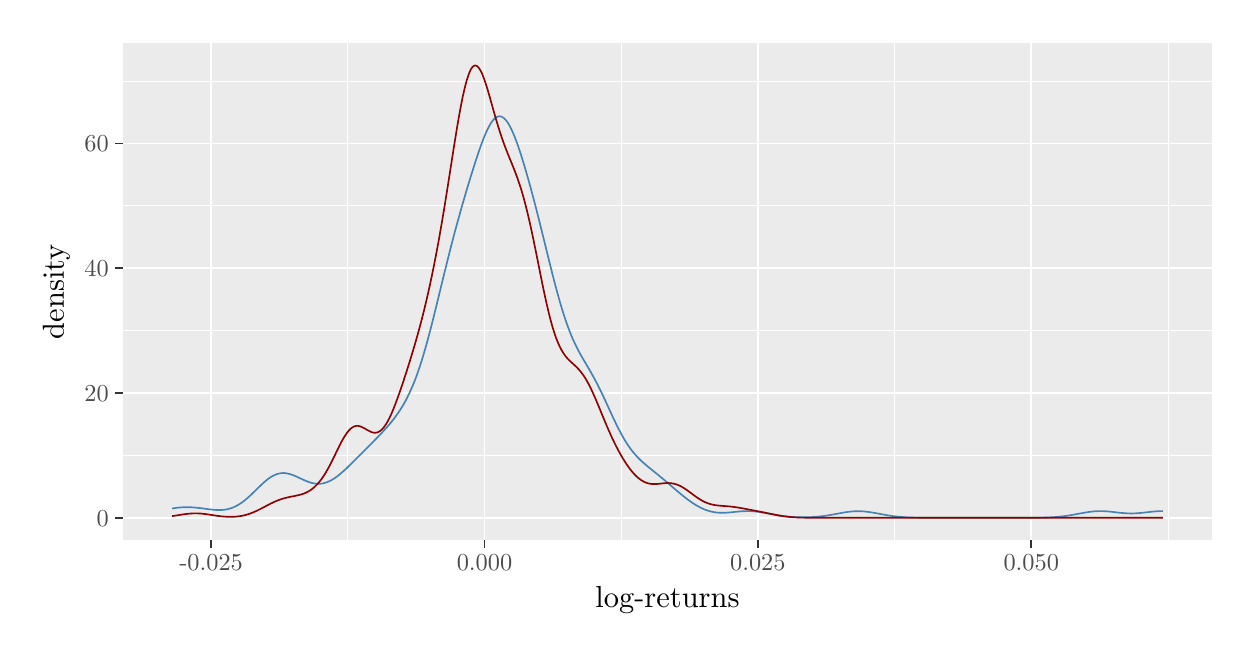
\begin{tikzpicture}[x=1pt,y=1pt]
\definecolor{fillColor}{RGB}{255,255,255}
\path[use as bounding box,fill=fillColor,fill opacity=0.00] (0,0) rectangle (433.62,216.81);
\begin{scope}
\path[clip] (  0.00,  0.00) rectangle (433.62,216.81);
\definecolor{drawColor}{RGB}{255,255,255}
\definecolor{fillColor}{RGB}{255,255,255}

\path[draw=drawColor,line width= 0.6pt,line join=round,line cap=round,fill=fillColor] (  0.00,  0.00) rectangle (433.62,216.81);
\end{scope}
\begin{scope}
\path[clip] ( 34.27, 31.53) rectangle (428.12,211.31);
\definecolor{fillColor}{gray}{0.92}

\path[fill=fillColor] ( 34.27, 31.53) rectangle (428.12,211.31);
\definecolor{drawColor}{RGB}{255,255,255}

\path[draw=drawColor,line width= 0.3pt,line join=round] ( 34.27, 62.24) --
	(428.12, 62.24);

\path[draw=drawColor,line width= 0.3pt,line join=round] ( 34.27,107.32) --
	(428.12,107.32);

\path[draw=drawColor,line width= 0.3pt,line join=round] ( 34.27,152.40) --
	(428.12,152.40);

\path[draw=drawColor,line width= 0.3pt,line join=round] ( 34.27,197.48) --
	(428.12,197.48);

\path[draw=drawColor,line width= 0.3pt,line join=round] (115.67, 31.53) --
	(115.67,211.31);

\path[draw=drawColor,line width= 0.3pt,line join=round] (214.46, 31.53) --
	(214.46,211.31);

\path[draw=drawColor,line width= 0.3pt,line join=round] (313.25, 31.53) --
	(313.25,211.31);

\path[draw=drawColor,line width= 0.3pt,line join=round] (412.03, 31.53) --
	(412.03,211.31);

\path[draw=drawColor,line width= 0.6pt,line join=round] ( 34.27, 39.70) --
	(428.12, 39.70);

\path[draw=drawColor,line width= 0.6pt,line join=round] ( 34.27, 84.78) --
	(428.12, 84.78);

\path[draw=drawColor,line width= 0.6pt,line join=round] ( 34.27,129.86) --
	(428.12,129.86);

\path[draw=drawColor,line width= 0.6pt,line join=round] ( 34.27,174.94) --
	(428.12,174.94);

\path[draw=drawColor,line width= 0.6pt,line join=round] ( 66.28, 31.53) --
	( 66.28,211.31);

\path[draw=drawColor,line width= 0.6pt,line join=round] (165.07, 31.53) --
	(165.07,211.31);

\path[draw=drawColor,line width= 0.6pt,line join=round] (263.85, 31.53) --
	(263.85,211.31);

\path[draw=drawColor,line width= 0.6pt,line join=round] (362.64, 31.53) --
	(362.64,211.31);
\definecolor{drawColor}{RGB}{70,130,180}

\path[draw=drawColor,line width= 0.6pt,line join=round] ( 52.17, 43.06) --
	( 52.87, 43.17) --
	( 53.57, 43.27) --
	( 54.27, 43.36) --
	( 54.97, 43.42) --
	( 55.67, 43.47) --
	( 56.37, 43.51) --
	( 57.07, 43.53) --
	( 57.78, 43.53) --
	( 58.48, 43.52) --
	( 59.18, 43.49) --
	( 59.88, 43.45) --
	( 60.58, 43.39) --
	( 61.28, 43.33) --
	( 61.98, 43.25) --
	( 62.68, 43.17) --
	( 63.38, 43.07) --
	( 64.08, 42.98) --
	( 64.78, 42.88) --
	( 65.48, 42.79) --
	( 66.18, 42.71) --
	( 66.88, 42.63) --
	( 67.59, 42.57) --
	( 68.29, 42.52) --
	( 68.99, 42.50) --
	( 69.69, 42.51) --
	( 70.39, 42.55) --
	( 71.09, 42.62) --
	( 71.79, 42.73) --
	( 72.49, 42.88) --
	( 73.19, 43.07) --
	( 73.89, 43.31) --
	( 74.59, 43.60) --
	( 75.29, 43.94) --
	( 75.99, 44.32) --
	( 76.69, 44.75) --
	( 77.39, 45.22) --
	( 78.10, 45.74) --
	( 78.80, 46.31) --
	( 79.50, 46.91) --
	( 80.20, 47.54) --
	( 80.90, 48.19) --
	( 81.60, 48.87) --
	( 82.30, 49.55) --
	( 83.00, 50.24) --
	( 83.70, 50.92) --
	( 84.40, 51.59) --
	( 85.10, 52.24) --
	( 85.80, 52.86) --
	( 86.50, 53.44) --
	( 87.20, 53.97) --
	( 87.90, 54.44) --
	( 88.61, 54.85) --
	( 89.31, 55.19) --
	( 90.01, 55.47) --
	( 90.71, 55.67) --
	( 91.41, 55.81) --
	( 92.11, 55.87) --
	( 92.81, 55.86) --
	( 93.51, 55.78) --
	( 94.21, 55.64) --
	( 94.91, 55.45) --
	( 95.61, 55.22) --
	( 96.31, 54.95) --
	( 97.01, 54.65) --
	( 97.71, 54.33) --
	( 98.42, 54.00) --
	( 99.12, 53.67) --
	( 99.82, 53.35) --
	(100.52, 53.05) --
	(101.22, 52.77) --
	(101.92, 52.52) --
	(102.62, 52.32) --
	(103.32, 52.16) --
	(104.02, 52.05) --
	(104.72, 51.99) --
	(105.42, 51.99) --
	(106.12, 52.05) --
	(106.82, 52.16) --
	(107.52, 52.35) --
	(108.22, 52.59) --
	(108.93, 52.89) --
	(109.63, 53.24) --
	(110.33, 53.64) --
	(111.03, 54.09) --
	(111.73, 54.59) --
	(112.43, 55.14) --
	(113.13, 55.71) --
	(113.83, 56.32) --
	(114.53, 56.95) --
	(115.23, 57.60) --
	(115.93, 58.27) --
	(116.63, 58.96) --
	(117.33, 59.65) --
	(118.03, 60.35) --
	(118.73, 61.05) --
	(119.44, 61.75) --
	(120.14, 62.46) --
	(120.84, 63.16) --
	(121.54, 63.86) --
	(122.24, 64.56) --
	(122.94, 65.26) --
	(123.64, 65.96) --
	(124.34, 66.67) --
	(125.04, 67.37) --
	(125.74, 68.09) --
	(126.44, 68.81) --
	(127.14, 69.53) --
	(127.84, 70.27) --
	(128.54, 71.03) --
	(129.24, 71.80) --
	(129.95, 72.59) --
	(130.65, 73.40) --
	(131.35, 74.24) --
	(132.05, 75.12) --
	(132.75, 76.04) --
	(133.45, 77.00) --
	(134.15, 78.01) --
	(134.85, 79.08) --
	(135.55, 80.22) --
	(136.25, 81.44) --
	(136.95, 82.75) --
	(137.65, 84.15) --
	(138.35, 85.65) --
	(139.05, 87.26) --
	(139.76, 88.97) --
	(140.46, 90.81) --
	(141.16, 92.79) --
	(141.86, 94.88) --
	(142.56, 97.09) --
	(143.26, 99.42) --
	(143.96,101.85) --
	(144.66,104.39) --
	(145.36,107.03) --
	(146.06,109.75) --
	(146.76,112.53) --
	(147.46,115.36) --
	(148.16,118.23) --
	(148.86,121.12) --
	(149.56,124.01) --
	(150.27,126.90) --
	(150.97,129.75) --
	(151.67,132.58) --
	(152.37,135.37) --
	(153.07,138.11) --
	(153.77,140.80) --
	(154.47,143.44) --
	(155.17,146.02) --
	(155.87,148.55) --
	(156.57,151.04) --
	(157.27,153.49) --
	(157.97,155.89) --
	(158.67,158.27) --
	(159.37,160.60) --
	(160.07,162.90) --
	(160.78,165.16) --
	(161.48,167.38) --
	(162.18,169.55) --
	(162.88,171.65) --
	(163.58,173.67) --
	(164.28,175.59) --
	(164.98,177.37) --
	(165.68,179.02) --
	(166.38,180.49) --
	(167.08,181.79) --
	(167.78,182.88) --
	(168.48,183.75) --
	(169.18,184.37) --
	(169.88,184.71) --
	(170.59,184.79) --
	(171.29,184.62) --
	(171.99,184.20) --
	(172.69,183.53) --
	(173.39,182.63) --
	(174.09,181.47) --
	(174.79,180.10) --
	(175.49,178.53) --
	(176.19,176.81) --
	(176.89,174.93) --
	(177.59,172.91) --
	(178.29,170.78) --
	(178.99,168.54) --
	(179.69,166.20) --
	(180.39,163.78) --
	(181.10,161.30) --
	(181.80,158.75) --
	(182.50,156.14) --
	(183.20,153.48) --
	(183.90,150.77) --
	(184.60,148.01) --
	(185.30,145.21) --
	(186.00,142.39) --
	(186.70,139.55) --
	(187.40,136.70) --
	(188.10,133.85) --
	(188.80,131.02) --
	(189.50,128.23) --
	(190.20,125.49) --
	(190.90,122.83) --
	(191.61,120.24) --
	(192.31,117.75) --
	(193.01,115.37) --
	(193.71,113.13) --
	(194.41,111.01) --
	(195.11,109.02) --
	(195.81,107.16) --
	(196.51,105.42) --
	(197.21,103.80) --
	(197.91,102.30) --
	(198.61,100.90) --
	(199.31, 99.57) --
	(200.01, 98.30) --
	(200.71, 97.07) --
	(201.42, 95.88) --
	(202.12, 94.69) --
	(202.82, 93.49) --
	(203.52, 92.28) --
	(204.22, 91.03) --
	(204.92, 89.74) --
	(205.62, 88.42) --
	(206.32, 87.04) --
	(207.02, 85.63) --
	(207.72, 84.17) --
	(208.42, 82.68) --
	(209.12, 81.16) --
	(209.82, 79.64) --
	(210.52, 78.11) --
	(211.22, 76.59) --
	(211.93, 75.09) --
	(212.63, 73.63) --
	(213.33, 72.22) --
	(214.03, 70.87) --
	(214.73, 69.57) --
	(215.43, 68.33) --
	(216.13, 67.17) --
	(216.83, 66.08) --
	(217.53, 65.07) --
	(218.23, 64.12) --
	(218.93, 63.25) --
	(219.63, 62.43) --
	(220.33, 61.66) --
	(221.03, 60.94) --
	(221.73, 60.27) --
	(222.44, 59.63) --
	(223.14, 59.02) --
	(223.84, 58.43) --
	(224.54, 57.85) --
	(225.24, 57.28) --
	(225.94, 56.71) --
	(226.64, 56.15) --
	(227.34, 55.59) --
	(228.04, 55.01) --
	(228.74, 54.44) --
	(229.44, 53.86) --
	(230.14, 53.27) --
	(230.84, 52.67) --
	(231.54, 52.08) --
	(232.24, 51.48) --
	(232.95, 50.87) --
	(233.65, 50.27) --
	(234.35, 49.67) --
	(235.05, 49.08) --
	(235.75, 48.50) --
	(236.45, 47.92) --
	(237.15, 47.36) --
	(237.85, 46.81) --
	(238.55, 46.28) --
	(239.25, 45.77) --
	(239.95, 45.28) --
	(240.65, 44.81) --
	(241.35, 44.37) --
	(242.05, 43.96) --
	(242.76, 43.58) --
	(243.46, 43.22) --
	(244.16, 42.90) --
	(244.86, 42.61) --
	(245.56, 42.36) --
	(246.26, 42.14) --
	(246.96, 41.96) --
	(247.66, 41.81) --
	(248.36, 41.69) --
	(249.06, 41.60) --
	(249.76, 41.54) --
	(250.46, 41.51) --
	(251.16, 41.50) --
	(251.86, 41.52) --
	(252.56, 41.56) --
	(253.27, 41.61) --
	(253.97, 41.67) --
	(254.67, 41.73) --
	(255.37, 41.81) --
	(256.07, 41.88) --
	(256.77, 41.95) --
	(257.47, 42.01) --
	(258.17, 42.05) --
	(258.87, 42.09) --
	(259.57, 42.12) --
	(260.27, 42.12) --
	(260.97, 42.11) --
	(261.67, 42.08) --
	(262.37, 42.03) --
	(263.07, 41.97) --
	(263.78, 41.89) --
	(264.48, 41.79) --
	(265.18, 41.69) --
	(265.88, 41.57) --
	(266.58, 41.45) --
	(267.28, 41.32) --
	(267.98, 41.19) --
	(268.68, 41.06) --
	(269.38, 40.93) --
	(270.08, 40.80) --
	(270.78, 40.68) --
	(271.48, 40.56) --
	(272.18, 40.46) --
	(272.88, 40.36) --
	(273.59, 40.27) --
	(274.29, 40.19) --
	(274.99, 40.12) --
	(275.69, 40.06) --
	(276.39, 40.01) --
	(277.09, 39.96) --
	(277.79, 39.93) --
	(278.49, 39.90) --
	(279.19, 39.89) --
	(279.89, 39.88) --
	(280.59, 39.88) --
	(281.29, 39.89) --
	(281.99, 39.90) --
	(282.69, 39.93) --
	(283.39, 39.96) --
	(284.10, 40.00) --
	(284.80, 40.05) --
	(285.50, 40.11) --
	(286.20, 40.18) --
	(286.90, 40.26) --
	(287.60, 40.35) --
	(288.30, 40.45) --
	(289.00, 40.55) --
	(289.70, 40.67) --
	(290.40, 40.79) --
	(291.10, 40.91) --
	(291.80, 41.04) --
	(292.50, 41.17) --
	(293.20, 41.30) --
	(293.90, 41.43) --
	(294.61, 41.56) --
	(295.31, 41.67) --
	(296.01, 41.78) --
	(296.71, 41.87) --
	(297.41, 41.95) --
	(298.11, 42.01) --
	(298.81, 42.06) --
	(299.51, 42.08) --
	(300.21, 42.09) --
	(300.91, 42.07) --
	(301.61, 42.04) --
	(302.31, 41.99) --
	(303.01, 41.92) --
	(303.71, 41.83) --
	(304.41, 41.73) --
	(305.12, 41.62) --
	(305.82, 41.50) --
	(306.52, 41.38) --
	(307.22, 41.25) --
	(307.92, 41.12) --
	(308.62, 40.99) --
	(309.32, 40.86) --
	(310.02, 40.73) --
	(310.72, 40.61) --
	(311.42, 40.50) --
	(312.12, 40.40) --
	(312.82, 40.30) --
	(313.52, 40.22) --
	(314.22, 40.14) --
	(314.93, 40.07) --
	(315.63, 40.01) --
	(316.33, 39.96) --
	(317.03, 39.91) --
	(317.73, 39.87) --
	(318.43, 39.84) --
	(319.13, 39.81) --
	(319.83, 39.79) --
	(320.53, 39.77) --
	(321.23, 39.76) --
	(321.93, 39.74) --
	(322.63, 39.73) --
	(323.33, 39.73) --
	(324.03, 39.72) --
	(324.73, 39.72) --
	(325.44, 39.71) --
	(326.14, 39.71) --
	(326.84, 39.71) --
	(327.54, 39.71) --
	(328.24, 39.71) --
	(328.94, 39.70) --
	(329.64, 39.70) --
	(330.34, 39.70) --
	(331.04, 39.70) --
	(331.74, 39.70) --
	(332.44, 39.70) --
	(333.14, 39.70) --
	(333.84, 39.70) --
	(334.54, 39.70) --
	(335.24, 39.70) --
	(335.95, 39.70) --
	(336.65, 39.70) --
	(337.35, 39.70) --
	(338.05, 39.70) --
	(338.75, 39.70) --
	(339.45, 39.70) --
	(340.15, 39.70) --
	(340.85, 39.70) --
	(341.55, 39.70) --
	(342.25, 39.70) --
	(342.95, 39.70) --
	(343.65, 39.70) --
	(344.35, 39.70) --
	(345.05, 39.70) --
	(345.76, 39.70) --
	(346.46, 39.70) --
	(347.16, 39.70) --
	(347.86, 39.70) --
	(348.56, 39.70) --
	(349.26, 39.70) --
	(349.96, 39.70) --
	(350.66, 39.70) --
	(351.36, 39.70) --
	(352.06, 39.70) --
	(352.76, 39.70) --
	(353.46, 39.70) --
	(354.16, 39.70) --
	(354.86, 39.70) --
	(355.56, 39.70) --
	(356.27, 39.70) --
	(356.97, 39.70) --
	(357.67, 39.70) --
	(358.37, 39.70) --
	(359.07, 39.71) --
	(359.77, 39.71) --
	(360.47, 39.71) --
	(361.17, 39.71) --
	(361.87, 39.71) --
	(362.57, 39.72) --
	(363.27, 39.72) --
	(363.97, 39.73) --
	(364.67, 39.73) --
	(365.37, 39.74) --
	(366.07, 39.75) --
	(366.78, 39.77) --
	(367.48, 39.79) --
	(368.18, 39.81) --
	(368.88, 39.84) --
	(369.58, 39.87) --
	(370.28, 39.90) --
	(370.98, 39.95) --
	(371.68, 40.00) --
	(372.38, 40.06) --
	(373.08, 40.13) --
	(373.78, 40.21) --
	(374.48, 40.29) --
	(375.18, 40.38) --
	(375.88, 40.49) --
	(376.58, 40.60) --
	(377.29, 40.72) --
	(377.99, 40.84) --
	(378.69, 40.97) --
	(379.39, 41.10) --
	(380.09, 41.23) --
	(380.79, 41.36) --
	(381.49, 41.49) --
	(382.19, 41.61) --
	(382.89, 41.72) --
	(383.59, 41.83) --
	(384.29, 41.92) --
	(384.99, 41.99) --
	(385.69, 42.05) --
	(386.39, 42.09) --
	(387.10, 42.11) --
	(387.80, 42.12) --
	(388.50, 42.11) --
	(389.20, 42.08) --
	(389.90, 42.03) --
	(390.60, 41.97) --
	(391.30, 41.91) --
	(392.00, 41.83) --
	(392.70, 41.75) --
	(393.40, 41.67) --
	(394.10, 41.59) --
	(394.80, 41.51) --
	(395.50, 41.44) --
	(396.20, 41.38) --
	(396.90, 41.34) --
	(397.61, 41.30) --
	(398.31, 41.28) --
	(399.01, 41.28) --
	(399.71, 41.29) --
	(400.41, 41.32) --
	(401.11, 41.37) --
	(401.81, 41.42) --
	(402.51, 41.49) --
	(403.21, 41.56) --
	(403.91, 41.64) --
	(404.61, 41.72) --
	(405.31, 41.80) --
	(406.01, 41.88) --
	(406.71, 41.95) --
	(407.41, 42.01) --
	(408.12, 42.06) --
	(408.82, 42.10) --
	(409.52, 42.11) --
	(410.22, 42.11);
\definecolor{drawColor}{RGB}{139,0,0}

\path[draw=drawColor,line width= 0.6pt,line join=round] ( 52.17, 40.31) --
	( 52.87, 40.41) --
	( 53.57, 40.51) --
	( 54.27, 40.63) --
	( 54.97, 40.74) --
	( 55.67, 40.85) --
	( 56.37, 40.95) --
	( 57.07, 41.05) --
	( 57.78, 41.14) --
	( 58.48, 41.21) --
	( 59.18, 41.26) --
	( 59.88, 41.30) --
	( 60.58, 41.31) --
	( 61.28, 41.30) --
	( 61.98, 41.27) --
	( 62.68, 41.22) --
	( 63.38, 41.15) --
	( 64.08, 41.07) --
	( 64.78, 40.98) --
	( 65.48, 40.88) --
	( 66.18, 40.77) --
	( 66.88, 40.66) --
	( 67.59, 40.55) --
	( 68.29, 40.45) --
	( 68.99, 40.35) --
	( 69.69, 40.27) --
	( 70.39, 40.19) --
	( 71.09, 40.13) --
	( 71.79, 40.09) --
	( 72.49, 40.06) --
	( 73.19, 40.05) --
	( 73.89, 40.06) --
	( 74.59, 40.09) --
	( 75.29, 40.13) --
	( 75.99, 40.21) --
	( 76.69, 40.30) --
	( 77.39, 40.42) --
	( 78.10, 40.57) --
	( 78.80, 40.74) --
	( 79.50, 40.94) --
	( 80.20, 41.17) --
	( 80.90, 41.43) --
	( 81.60, 41.71) --
	( 82.30, 42.02) --
	( 83.00, 42.34) --
	( 83.70, 42.69) --
	( 84.40, 43.04) --
	( 85.10, 43.41) --
	( 85.80, 43.78) --
	( 86.50, 44.16) --
	( 87.20, 44.52) --
	( 87.90, 44.88) --
	( 88.61, 45.22) --
	( 89.31, 45.54) --
	( 90.01, 45.84) --
	( 90.71, 46.12) --
	( 91.41, 46.37) --
	( 92.11, 46.59) --
	( 92.81, 46.79) --
	( 93.51, 46.97) --
	( 94.21, 47.13) --
	( 94.91, 47.28) --
	( 95.61, 47.42) --
	( 96.31, 47.55) --
	( 97.01, 47.70) --
	( 97.71, 47.85) --
	( 98.42, 48.03) --
	( 99.12, 48.24) --
	( 99.82, 48.48) --
	(100.52, 48.77) --
	(101.22, 49.11) --
	(101.92, 49.51) --
	(102.62, 49.99) --
	(103.32, 50.55) --
	(104.02, 51.18) --
	(104.72, 51.91) --
	(105.42, 52.72) --
	(106.12, 53.63) --
	(106.82, 54.63) --
	(107.52, 55.72) --
	(108.22, 56.92) --
	(108.93, 58.20) --
	(109.63, 59.55) --
	(110.33, 60.95) --
	(111.03, 62.38) --
	(111.73, 63.83) --
	(112.43, 65.26) --
	(113.13, 66.64) --
	(113.83, 67.95) --
	(114.53, 69.14) --
	(115.23, 70.20) --
	(115.93, 71.10) --
	(116.63, 71.83) --
	(117.33, 72.37) --
	(118.03, 72.73) --
	(118.73, 72.91) --
	(119.44, 72.91) --
	(120.14, 72.74) --
	(120.84, 72.47) --
	(121.54, 72.11) --
	(122.24, 71.71) --
	(122.94, 71.30) --
	(123.64, 70.94) --
	(124.34, 70.64) --
	(125.04, 70.45) --
	(125.74, 70.43) --
	(126.44, 70.58) --
	(127.14, 70.92) --
	(127.84, 71.46) --
	(128.54, 72.21) --
	(129.24, 73.15) --
	(129.95, 74.29) --
	(130.65, 75.61) --
	(131.35, 77.10) --
	(132.05, 78.74) --
	(132.75, 80.51) --
	(133.45, 82.37) --
	(134.15, 84.32) --
	(134.85, 86.33) --
	(135.55, 88.41) --
	(136.25, 90.53) --
	(136.95, 92.69) --
	(137.65, 94.90) --
	(138.35, 97.16) --
	(139.05, 99.47) --
	(139.76,101.83) --
	(140.46,104.26) --
	(141.16,106.77) --
	(141.86,109.35) --
	(142.56,112.03) --
	(143.26,114.81) --
	(143.96,117.72) --
	(144.66,120.75) --
	(145.36,123.90) --
	(146.06,127.19) --
	(146.76,130.62) --
	(147.46,134.19) --
	(148.16,137.92) --
	(148.86,141.79) --
	(149.56,145.83) --
	(150.27,150.01) --
	(150.97,154.30) --
	(151.67,158.70) --
	(152.37,163.16) --
	(153.07,167.65) --
	(153.77,172.13) --
	(154.47,176.54) --
	(155.17,180.82) --
	(155.87,184.88) --
	(156.57,188.67) --
	(157.27,192.14) --
	(157.97,195.21) --
	(158.67,197.85) --
	(159.37,199.99) --
	(160.07,201.62) --
	(160.78,202.68) --
	(161.48,203.14) --
	(162.18,203.06) --
	(162.88,202.48) --
	(163.58,201.44) --
	(164.28,199.99) --
	(164.98,198.18) --
	(165.68,196.10) --
	(166.38,193.80) --
	(167.08,191.36) --
	(167.78,188.85) --
	(168.48,186.35) --
	(169.18,183.90) --
	(169.88,181.54) --
	(170.59,179.29) --
	(171.29,177.16) --
	(171.99,175.16) --
	(172.69,173.29) --
	(173.39,171.50) --
	(174.09,169.78) --
	(174.79,168.07) --
	(175.49,166.34) --
	(176.19,164.55) --
	(176.89,162.67) --
	(177.59,160.66) --
	(178.29,158.49) --
	(178.99,156.12) --
	(179.69,153.55) --
	(180.39,150.78) --
	(181.10,147.83) --
	(181.80,144.71) --
	(182.50,141.44) --
	(183.20,138.05) --
	(183.90,134.58) --
	(184.60,131.07) --
	(185.30,127.57) --
	(186.00,124.13) --
	(186.70,120.79) --
	(187.40,117.59) --
	(188.10,114.57) --
	(188.80,111.75) --
	(189.50,109.17) --
	(190.20,106.84) --
	(190.90,104.80) --
	(191.61,103.01) --
	(192.31,101.45) --
	(193.01,100.13) --
	(193.71, 99.00) --
	(194.41, 98.04) --
	(195.11, 97.22) --
	(195.81, 96.50) --
	(196.51, 95.85) --
	(197.21, 95.22) --
	(197.91, 94.57) --
	(198.61, 93.88) --
	(199.31, 93.13) --
	(200.01, 92.28) --
	(200.71, 91.33) --
	(201.42, 90.27) --
	(202.12, 89.09) --
	(202.82, 87.79) --
	(203.52, 86.38) --
	(204.22, 84.88) --
	(204.92, 83.31) --
	(205.62, 81.68) --
	(206.32, 80.01) --
	(207.02, 78.31) --
	(207.72, 76.60) --
	(208.42, 74.91) --
	(209.12, 73.24) --
	(209.82, 71.61) --
	(210.52, 70.03) --
	(211.22, 68.49) --
	(211.93, 67.02) --
	(212.63, 65.60) --
	(213.33, 64.24) --
	(214.03, 62.95) --
	(214.73, 61.73) --
	(215.43, 60.57) --
	(216.13, 59.48) --
	(216.83, 58.45) --
	(217.53, 57.49) --
	(218.23, 56.59) --
	(218.93, 55.77) --
	(219.63, 55.03) --
	(220.33, 54.37) --
	(221.03, 53.79) --
	(221.73, 53.29) --
	(222.44, 52.87) --
	(223.14, 52.53) --
	(223.84, 52.27) --
	(224.54, 52.08) --
	(225.24, 51.96) --
	(225.94, 51.90) --
	(226.64, 51.90) --
	(227.34, 51.93) --
	(228.04, 51.99) --
	(228.74, 52.06) --
	(229.44, 52.14) --
	(230.14, 52.20) --
	(230.84, 52.25) --
	(231.54, 52.26) --
	(232.24, 52.22) --
	(232.95, 52.13) --
	(233.65, 51.99) --
	(234.35, 51.79) --
	(235.05, 51.54) --
	(235.75, 51.22) --
	(236.45, 50.85) --
	(237.15, 50.43) --
	(237.85, 49.97) --
	(238.55, 49.47) --
	(239.25, 48.96) --
	(239.95, 48.44) --
	(240.65, 47.92) --
	(241.35, 47.41) --
	(242.05, 46.92) --
	(242.76, 46.46) --
	(243.46, 46.03) --
	(244.16, 45.66) --
	(244.86, 45.32) --
	(245.56, 45.03) --
	(246.26, 44.79) --
	(246.96, 44.59) --
	(247.66, 44.42) --
	(248.36, 44.29) --
	(249.06, 44.19) --
	(249.76, 44.12) --
	(250.46, 44.06) --
	(251.16, 44.00) --
	(251.86, 43.95) --
	(252.56, 43.90) --
	(253.27, 43.84) --
	(253.97, 43.77) --
	(254.67, 43.69) --
	(255.37, 43.60) --
	(256.07, 43.50) --
	(256.77, 43.39) --
	(257.47, 43.27) --
	(258.17, 43.15) --
	(258.87, 43.02) --
	(259.57, 42.89) --
	(260.27, 42.75) --
	(260.97, 42.62) --
	(261.67, 42.49) --
	(262.37, 42.35) --
	(263.07, 42.22) --
	(263.78, 42.08) --
	(264.48, 41.95) --
	(265.18, 41.81) --
	(265.88, 41.67) --
	(266.58, 41.52) --
	(267.28, 41.37) --
	(267.98, 41.23) --
	(268.68, 41.08) --
	(269.38, 40.94) --
	(270.08, 40.80) --
	(270.78, 40.66) --
	(271.48, 40.53) --
	(272.18, 40.42) --
	(272.88, 40.31) --
	(273.59, 40.21) --
	(274.29, 40.12) --
	(274.99, 40.05) --
	(275.69, 39.98) --
	(276.39, 39.92) --
	(277.09, 39.88) --
	(277.79, 39.84) --
	(278.49, 39.80) --
	(279.19, 39.78) --
	(279.89, 39.76) --
	(280.59, 39.75) --
	(281.29, 39.73) --
	(281.99, 39.72) --
	(282.69, 39.72) --
	(283.39, 39.71) --
	(284.10, 39.71) --
	(284.80, 39.71) --
	(285.50, 39.71) --
	(286.20, 39.70) --
	(286.90, 39.70) --
	(287.60, 39.70) --
	(288.30, 39.70) --
	(289.00, 39.70) --
	(289.70, 39.70) --
	(290.40, 39.70) --
	(291.10, 39.70) --
	(291.80, 39.70) --
	(292.50, 39.70) --
	(293.20, 39.70) --
	(293.90, 39.70) --
	(294.61, 39.70) --
	(295.31, 39.70) --
	(296.01, 39.70) --
	(296.71, 39.70) --
	(297.41, 39.70) --
	(298.11, 39.70) --
	(298.81, 39.70) --
	(299.51, 39.70) --
	(300.21, 39.70) --
	(300.91, 39.70) --
	(301.61, 39.70) --
	(302.31, 39.70) --
	(303.01, 39.70) --
	(303.71, 39.70) --
	(304.41, 39.70) --
	(305.12, 39.70) --
	(305.82, 39.70) --
	(306.52, 39.70) --
	(307.22, 39.70) --
	(307.92, 39.70) --
	(308.62, 39.70) --
	(309.32, 39.70) --
	(310.02, 39.70) --
	(310.72, 39.70) --
	(311.42, 39.70) --
	(312.12, 39.70) --
	(312.82, 39.70) --
	(313.52, 39.70) --
	(314.22, 39.70) --
	(314.93, 39.70) --
	(315.63, 39.70) --
	(316.33, 39.70) --
	(317.03, 39.70) --
	(317.73, 39.70) --
	(318.43, 39.70) --
	(319.13, 39.70) --
	(319.83, 39.70) --
	(320.53, 39.70) --
	(321.23, 39.70) --
	(321.93, 39.70) --
	(322.63, 39.70) --
	(323.33, 39.70) --
	(324.03, 39.70) --
	(324.73, 39.70) --
	(325.44, 39.70) --
	(326.14, 39.70) --
	(326.84, 39.70) --
	(327.54, 39.70) --
	(328.24, 39.70) --
	(328.94, 39.70) --
	(329.64, 39.70) --
	(330.34, 39.70) --
	(331.04, 39.70) --
	(331.74, 39.70) --
	(332.44, 39.70) --
	(333.14, 39.70) --
	(333.84, 39.70) --
	(334.54, 39.70) --
	(335.24, 39.70) --
	(335.95, 39.70) --
	(336.65, 39.70) --
	(337.35, 39.70) --
	(338.05, 39.70) --
	(338.75, 39.70) --
	(339.45, 39.70) --
	(340.15, 39.70) --
	(340.85, 39.70) --
	(341.55, 39.70) --
	(342.25, 39.70) --
	(342.95, 39.70) --
	(343.65, 39.70) --
	(344.35, 39.70) --
	(345.05, 39.70) --
	(345.76, 39.70) --
	(346.46, 39.70) --
	(347.16, 39.70) --
	(347.86, 39.70) --
	(348.56, 39.70) --
	(349.26, 39.70) --
	(349.96, 39.70) --
	(350.66, 39.70) --
	(351.36, 39.70) --
	(352.06, 39.70) --
	(352.76, 39.70) --
	(353.46, 39.70) --
	(354.16, 39.70) --
	(354.86, 39.70) --
	(355.56, 39.70) --
	(356.27, 39.70) --
	(356.97, 39.70) --
	(357.67, 39.70) --
	(358.37, 39.70) --
	(359.07, 39.70) --
	(359.77, 39.70) --
	(360.47, 39.70) --
	(361.17, 39.70) --
	(361.87, 39.70) --
	(362.57, 39.70) --
	(363.27, 39.70) --
	(363.97, 39.70) --
	(364.67, 39.70) --
	(365.37, 39.70) --
	(366.07, 39.70) --
	(366.78, 39.70) --
	(367.48, 39.70) --
	(368.18, 39.70) --
	(368.88, 39.70) --
	(369.58, 39.70) --
	(370.28, 39.70) --
	(370.98, 39.70) --
	(371.68, 39.70) --
	(372.38, 39.70) --
	(373.08, 39.70) --
	(373.78, 39.70) --
	(374.48, 39.70) --
	(375.18, 39.70) --
	(375.88, 39.70) --
	(376.58, 39.70) --
	(377.29, 39.70) --
	(377.99, 39.70) --
	(378.69, 39.70) --
	(379.39, 39.70) --
	(380.09, 39.70) --
	(380.79, 39.70) --
	(381.49, 39.70) --
	(382.19, 39.70) --
	(382.89, 39.70) --
	(383.59, 39.70) --
	(384.29, 39.70) --
	(384.99, 39.70) --
	(385.69, 39.70) --
	(386.39, 39.70) --
	(387.10, 39.70) --
	(387.80, 39.70) --
	(388.50, 39.70) --
	(389.20, 39.70) --
	(389.90, 39.70) --
	(390.60, 39.70) --
	(391.30, 39.70) --
	(392.00, 39.70) --
	(392.70, 39.70) --
	(393.40, 39.70) --
	(394.10, 39.70) --
	(394.80, 39.70) --
	(395.50, 39.70) --
	(396.20, 39.70) --
	(396.90, 39.70) --
	(397.61, 39.70) --
	(398.31, 39.70) --
	(399.01, 39.70) --
	(399.71, 39.70) --
	(400.41, 39.70) --
	(401.11, 39.70) --
	(401.81, 39.70) --
	(402.51, 39.70) --
	(403.21, 39.70) --
	(403.91, 39.70) --
	(404.61, 39.70) --
	(405.31, 39.70) --
	(406.01, 39.70) --
	(406.71, 39.70) --
	(407.41, 39.70) --
	(408.12, 39.70) --
	(408.82, 39.70) --
	(409.52, 39.70) --
	(410.22, 39.70);
\end{scope}
\begin{scope}
\path[clip] (  0.00,  0.00) rectangle (433.62,216.81);
\definecolor{drawColor}{gray}{0.30}

\node[text=drawColor,anchor=base east,inner sep=0pt, outer sep=0pt, scale=  0.88] at ( 29.32, 36.67) {0};

\node[text=drawColor,anchor=base east,inner sep=0pt, outer sep=0pt, scale=  0.88] at ( 29.32, 81.75) {20};

\node[text=drawColor,anchor=base east,inner sep=0pt, outer sep=0pt, scale=  0.88] at ( 29.32,126.83) {40};

\node[text=drawColor,anchor=base east,inner sep=0pt, outer sep=0pt, scale=  0.88] at ( 29.32,171.91) {60};
\end{scope}
\begin{scope}
\path[clip] (  0.00,  0.00) rectangle (433.62,216.81);
\definecolor{drawColor}{gray}{0.20}

\path[draw=drawColor,line width= 0.6pt,line join=round] ( 31.52, 39.70) --
	( 34.27, 39.70);

\path[draw=drawColor,line width= 0.6pt,line join=round] ( 31.52, 84.78) --
	( 34.27, 84.78);

\path[draw=drawColor,line width= 0.6pt,line join=round] ( 31.52,129.86) --
	( 34.27,129.86);

\path[draw=drawColor,line width= 0.6pt,line join=round] ( 31.52,174.94) --
	( 34.27,174.94);
\end{scope}
\begin{scope}
\path[clip] (  0.00,  0.00) rectangle (433.62,216.81);
\definecolor{drawColor}{gray}{0.20}

\path[draw=drawColor,line width= 0.6pt,line join=round] ( 66.28, 28.78) --
	( 66.28, 31.53);

\path[draw=drawColor,line width= 0.6pt,line join=round] (165.07, 28.78) --
	(165.07, 31.53);

\path[draw=drawColor,line width= 0.6pt,line join=round] (263.85, 28.78) --
	(263.85, 31.53);

\path[draw=drawColor,line width= 0.6pt,line join=round] (362.64, 28.78) --
	(362.64, 31.53);
\end{scope}
\begin{scope}
\path[clip] (  0.00,  0.00) rectangle (433.62,216.81);
\definecolor{drawColor}{gray}{0.30}

\node[text=drawColor,anchor=base,inner sep=0pt, outer sep=0pt, scale=  0.88] at ( 66.28, 20.52) {-0.025};

\node[text=drawColor,anchor=base,inner sep=0pt, outer sep=0pt, scale=  0.88] at (165.07, 20.52) {0.000};

\node[text=drawColor,anchor=base,inner sep=0pt, outer sep=0pt, scale=  0.88] at (263.85, 20.52) {0.025};

\node[text=drawColor,anchor=base,inner sep=0pt, outer sep=0pt, scale=  0.88] at (362.64, 20.52) {0.050};
\end{scope}
\begin{scope}
\path[clip] (  0.00,  0.00) rectangle (433.62,216.81);
\definecolor{drawColor}{RGB}{0,0,0}

\node[text=drawColor,anchor=base,inner sep=0pt, outer sep=0pt, scale=  1.10] at (231.19,  7.44) {log-returns};
\end{scope}
\begin{scope}
\path[clip] (  0.00,  0.00) rectangle (433.62,216.81);
\definecolor{drawColor}{RGB}{0,0,0}

\node[text=drawColor,rotate= 90.00,anchor=base,inner sep=0pt, outer sep=0pt, scale=  1.10] at ( 13.08,121.42) {density};
\end{scope}
\end{tikzpicture}

  \caption{Historical and HSV related Apple stock Log-returns distribution}
  \floatfoot{The above blue density curve is constructed over the historical data of the Apple share of stock price evolution from 18th May 2017 to 18th May 2018. while the red curve is constructed from time-series genereated by the function \textit{hsv\_ts} taking the risk-neutral parameters \ref{eq:methodology:arg:heston:riskneutral} as arguments.
  }
  \label{p:methodology:density:aapl:heston:riskneutral}
\end{figure}


The goal of that section is to find the parameters that make the distributions of the log-returns generated from market data or from \textit{HSV\_ts()} fit together.
To do so, and according to the differences between \cref{eq:other:hsvstock:riskless,eq:other:hsvvol:riskless} from \cref{eq:other:hsvstock,eq:other:hsvvol}, the parameters to modify are the drift rate $r \to \alpha$, the mean reversion speed $\kappa^{*} \to \kappa$ and the long-run volatility $\theta^* \to \theta$.
Accordingly, the correlation parameter $\rho$ and the volatility of the volatility $\sigma$ stay unchanged from  the risk-neutral to risk-averse world.

I followed the method exhibited at \cref{sec:upstream:logreturn} to get a rough estimate of the drift rate $\alpha$. From the log-returns' first and second moments, I find the value 0.4822917 as the estimation of $\alpha$.

According to \cref{eq:other:kappa:riskless,eq:other:theta:riskless}, in order to  calculate $\kappa$ and $\theta$, the risk premium $\lambda$ has to be estimated.
Practically, to do so, I am using an approximation algorithm developed by \cite{MASS} which is directly available in R through the function \textit{fitdistr} from the R package \textit{MASS}. 
To do the job, that algorithm needs (i) a density function to be fitted along with (ii) a sample of random data as a template.
As defined in \citet{Adrian}, the density of the log-return generated by the HSV model is given by \cref{methodology:density:heston:log}.

\begin{align}
P_t(x) &= \frac{1}{2 \pi} \int_{-\infty}^{\infty} e^{i \phi x + F_t(\phi)} d\phi \label{methodology:density:heston:log} \\
\intertext{where}
F_t(\phi) &= \frac{\kappa \theta}{\sigma^2} \gamma t -
  \frac{2 \kappa \theta}{\sigma ^2} \ln\left(
    \cosh \frac{\omega t}{2} +
    \frac{\omega^2 - \gamma^2 +2 \kappa \gamma}{2 \kappa \omega} \sinh \frac{\omega t}{2}
  \right) \notag \\
\intertext{and}
\omega &= \sqrt{\gamma^2 + \sigma^2 (\phi^2 - i\phi)}, \notag
\gamma = \kappa + i \rho \phi \sigma \notag
\end{align}

By applying the optimization function together with \cref{methodology:density:heston:log} as a density function, data [REF] as template and the variable $\lambda$ as a cursor, the optimization algorithm outputs $\lambda = 4.7883278229$ as best fit arguments for the risk premium.
Therefore, the set of the "risk-averse" parameters is fully described here below in \ref{eq:methodology:arg:heston:riskaverse}.

\begin{align}
  \left \{
  \begin{array}{lcl}
    V(0) &= &0.03798218, \\
    \theta &= &0.02217598, \\
    \sigma &= &0.50378803, \\
    \rho &= &-0.39877827, \\
    \kappa &= &8.789383, \\
    \alpha & = &0.4822917
  \end{array}
  \right \}  
  \label{eq:methodology:arg:heston:riskaverse}
\end{align}

FIGURE shows the distribution of the HSV related log-returns with respect to the distribution of those computed from the market.

[FIGURE]

Consequently, the set \ref{eq:methodology:arg:heston:riskaverse} is the one I will use together with the \textit{HSV\_ts()} function whenever I have to compute time series using the HSV model and within the real world constraints.


















% \SweaveInput{appendix}









\bibliography{bibl}
\bibliographystyle{plainnat}
\end{document}
